\chapter{Interpretation of Search Results}
\label{sec:interpretation}
\section{Introduction}
It is very often the case that a search for \ac{NP} will yield results
consistent with the currently accepted theory (which, in most particle physics
contexts would be the \ac{SM}). In the absence of a discovery, it is often
desirable to provide additional information in the form of a statistical
interpretation of the results. Such an interpretation typically serves the
following goals.
\begin{itemize}
\item To indicate the sensitivity of the analysis to the proposed model or set
  of models. This can then be used as an objective measure by which to compare
  different analyses or to benchmark the progress of a single analysis as data
  is collected.
\item To falsify,, to some confidence level, a particular theory or some region
  of parameter space within that theory.
\item To guide the choice of analysis cuts and object selection requirements.
\end{itemize}

Providing an interpretation invariably necessitates some choice of theory or
phenomenological model against which to test the results. The range of theories
will of course depend strongly on the inclusiveness of the experiment. Indeed,
in many cases a single theory will have motivated the analysis in the first
place and the choice of model will be clear. In other cases, the analysis has
been designed to be as inclusive as possible and therefore sensitive to an array
of theories. Typically this is achieved by focussing on a particular detector
signature (for instance missing transverse energy), where a deviation from the
\ac{SM} is a common feature of many \ac{NP} scenarios.

As was seen in \chap~\ref{sec:framework}, \ac{LHC} searches have typically
interpreted the results of \ac{SUSY} searches in the context of the
\ac{CMSSM}. This provides a convenient benchmark space for the comparison of
different searches. However, it restricts the range of physics signatures rather
more than is desirable. It was seen that by selecting models from a spectrum of
simplified models, searches can provide more generic and useful interpretations
of their results.

This chapter will describe the statistical methods used to interpret the results
of the single lepton search. These will then be applied to the \ac{CMSSM} and to
the two simplified models described in \chap~\ref{sec:framework}: \TthreeW and
\Ttwott.

\section{Statistical Methods}
\subsection{The Likelihood Function}
Consider some statistical model, believed to describe a set of experimental data
and depending on a set of parameters, $\theta$. The \emph{likelihood} of given
values of $\theta$ in light of experimental observations, $X$, is the
probability of observing $X$ given
$\theta$~\cite{statistical_methods,louis_lyons}. Considered as a function of the parameter
$\theta$ given experimental measurements, $X$, the likelihood may be written
\begin{equation}
\label{eqn:inter_likelihood}
\likelihood\left(\theta|X\right) = P\left(X|\theta\right),
\end{equation}
where $P\left(X|\theta\right)$ should be read as ``the probability of $X$ given
$\theta$''.

Likelihood functions are an important tool in comparing theoretical expectations
to experiment. Often, two proposed values for the parameter $\theta$ will be
compared using the \emph{likelihood ratio},
\begin{equation}
\label{eqn:inter_likelihood_ratio}
  \likelihoodratio = \frac{\likelihood\left(\theta_1|X\right)}{\likelihood\left(\theta_2|X\right)} = \frac{\alpha P\left(X|\theta_1\right)}{\alpha P\left(X|\theta_2\right)}.
\end{equation}
Here, the numerator and denominator are related to
\eqn~\ref{eqn:inter_likelihood} by a constant $\alpha$. Here, as in many uses of
the likelihood function, such constant factors can be safely ignored.  This is
known as a \emph{likelihood ratio test} and may be used to compare two
hypotheses.

An important use of the likelihood function is in estimation of the parameters
$\theta$ given some set of observations. The value of $\theta$ which maximises
$\likelihood$ is known as the \acf{MLE} of $\theta$, denoted
$\hat{\theta}$. Often it will be convenient to work with the logarithm of the
likelihood function, $\ln\likelihood$. Since the logarithm is a monotonically
increasing function, its maxima coincide with those of $\likelihood$.


\subsection{Profile Likelihood and Wilks' Theorem}
\label{sec:inter_profile_likelihood}
The likelihood function for a complex experiment may depend on a large number of
free parameters. A number of these may be introduced to describe experimental
effects such as backgrounds or uncertainties which are not directly relevant to
the underlying measurement. These are known as \emph{nuisance parameters}. In
contrast, the parameters to be measured by the experiment are known as
\emph{parameters of interest}.

The full likelihood function may be reduced to a \emph{profile likelihood}, by
rewriting the nuisance parameters in terms of the parameters of interest. The
profile likelihood ratio is defined as
\begin{equation*}
  \lambda = \frac{\likelihood\left(\mu, \hat{\hat{\nu}}\left(\mu\right)\right)}{\likelihood\left(\hat{\mu}, \hat{\nu}\right)},
\end{equation*}
where $\mu$ are the parameters of interest and $\nu$ the nuisance
parameters. $\hat{\mu}$ and $\hat{\nu}$ are the \acp{MLE} of $\mu$ and $\nu$
respectively. $\hat{\hat{\nu}}$ is the \emph{conditional} \ac{MLE} of $\nu$ -
the \ac{MLE} of $\nu$ for a given value of $\mu$.

It is frequently the case that, in addition to calculating a maximum-likelihood
estimate for a given parameter, it is also desirable to estimate a range in
which the ``true'' value of the parameter can be said to lie with a given degree
of certainty. This procedure is known as \emph{interval estimation}, and the
resulting interval, a \emph{confidence interval}.

Wilks' theorem states that $-2\ln\likelihoodratio$ is distributed as a $\chi^2$
distribution~\cite{statistical_methods,param_estimation}. The number of degrees
of freedom of this distribution is determined by the difference in the number of
free parameters in the numerator and denominator of the likelihood ratio
($\theta_1$ and $\theta_2$ in \eqn~\ref{eqn:inter_likelihood_ratio}). In the
case of the profile likelihood ratio, this is equal to the number of parameters
of interest, $\mu$. Wilks' theorem can therefore be used to provide an interval
estimate for the parameters of interest $\mu$. This method will be referred to
as the \ac{PL} method.

\subsection{Hypothesis Testing}
\label{sec:inter_cls}
It has been seen that the likelihood ratio may be used to compare two hypotheses
$H_0$ and $H_1$. Typically $H_0$ will be referred to as the ``null hypothesis''
and $H_1$, the ``alternate hypothesis''. For a given hypothesis $H$ and
observation, $X$, the \emph{p-value} gives the probability of making a
measurement as consistent or less with the hypothesis $H$, than
$X$~\cite{statistical_methods}.

There are a variety of techniques for choosing between competing
hypotheses. Typically, a certain test statistic is used -- for instance the
number of signal events observed or the likelihood ratio. For a given
hypothesis, a critical region $W$, can be defined where the probability of
making such an observation, assuming the hypothesis, is below some threshold,
$\alpha$,
\begin{equation*}
P\left(x \in W|H\right) \leq \alpha,
\end{equation*}
where $x$ is the test statistic. $\alpha$ is often chosen as 0.05. Then, if the
measured value of $x$ is found to be in the critical region, the hypothesis $H$
can be said to be rejected with 95\% confidence.

One way to define such an interval is to run toy \ac{MC} experiments to
generate the distributions of the test statistic corresponding to the null and
alternate hypotheses. It is then straightforward to define the critical region
as that point at which the p-value reaches a suitably low threshold, say
$0.05$. This is illustrated in \fig~\ref{fig:inter_cls_explain1}.

\begin{figure}[h!]
\centering
\subfloat[]{\label{fig:inter_cls_explain1}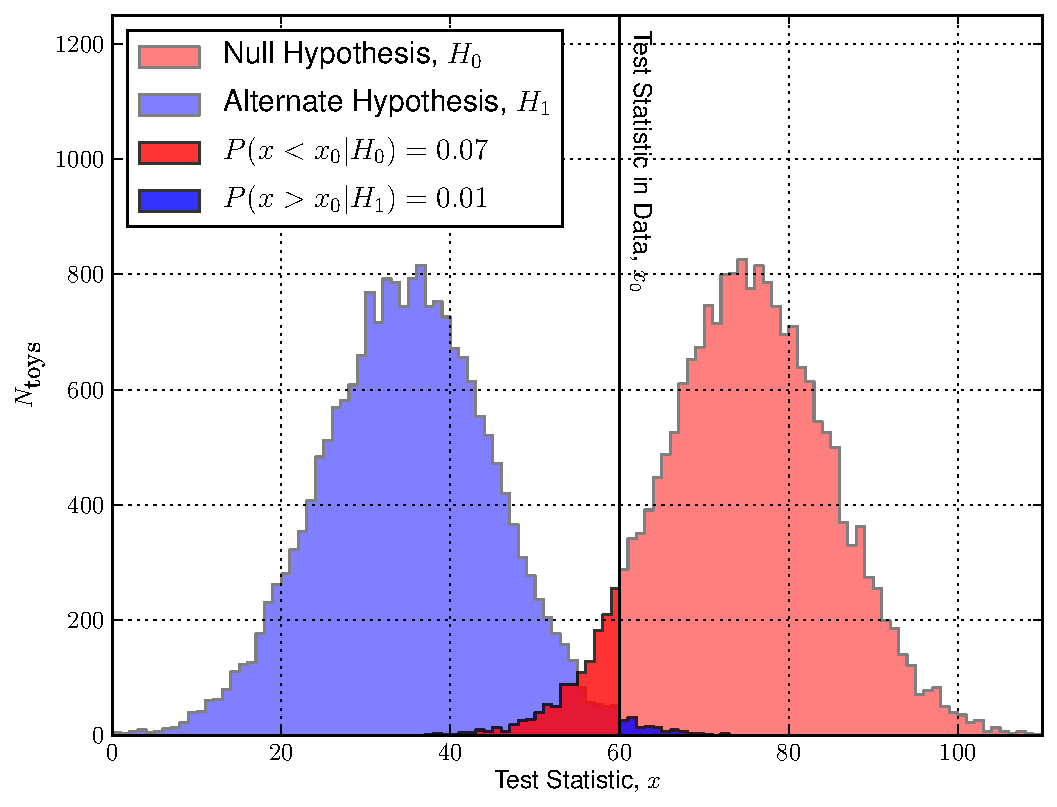
\includegraphics[width=0.49\textwidth]{fig/cls1}}
\subfloat[]{\label{fig:inter_cls_explain2}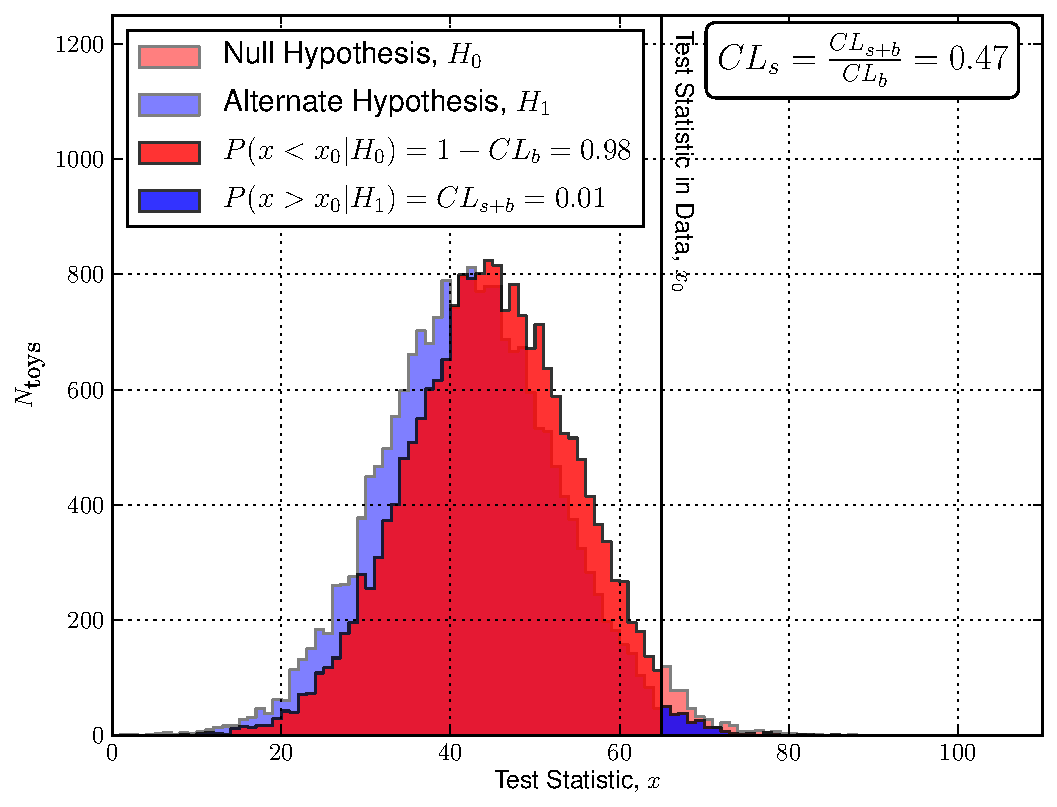
\includegraphics[width=0.49\textwidth]{fig/cls2}}
\caption[Illustration showing the use of the \CLs method]{Illustration showing
  the use of the \CLs method. \subref{fig:inter_cls_explain1} shows the
  evaluation of a p-value in the presence of two hypotheses, well-separated in
  the test statistic. \subref{fig:inter_cls_explain2} shows the case where the
  null and alternate hypothesis are not well separated. In this case, the
  calculation of \CLs is shown.}
\label{fig:inter_cls_explain}
\end{figure}

\subsection[The \CLs Method]{The \boldmath{\CLs} Method}
One deficiency of the above method is that often the two hypotheses will not be
so well separated. This situation is shown in
\fig~\ref{fig:inter_cls_explain2}. In this case, the p-value for the alternate
hypothesis is small and so would result in an exclusion. This is undesirable
since the test statistic is clearly not sensitive enough to distinguish between
the two hypotheses.

To address this problem, the \CLs hypothesis test may be used instead~\cite{cls,confidence_level},
\begin{equation*}
\CLs = \frac{CLspb}{CLb},
\end{equation*}
where, for the example shown in \fig~\ref{fig:inter_cls_explain2},
\begin{eqnarray*}
CLspb = P\left(x > x_0 | H_1\right)\\
CLb = 1 - P\left(x < x_0 | H_0\right),
\end{eqnarray*}
and the null hypothesis now represents a background-only scenario, b, and the
alternate, signal-plus-background, s+b. Using the \CLs to test the alternate
hypothesis, instead of a p-value, penalises cases where the test statistic
provides little sensitivity -- since \CLb will be large. For a 95\% exclusion,
$\CLs < 0.05$ is required as before. The \CLs method may also be used to derive
an upper limit on some parameter by scanning through a range of values of the
parameter of interest in order to obtain a 95\% upper limit. This is known as
``hypothesis test inversion''.

Several additional details are relevant to the discussion here. For the toy
experiments used to generate the test statistic distributions, the nuisance
parameters are each sampled randomly according to their expected
distributions. This ensures that the full range of their uncertainties is
covered. The test statistic that has been used is the one-sided profile
likelihood ratio,
$\qmu=-2\ln\lambda$~\cite{cl_computation,modified_frequentist,atlas_cms_higgs,cl_asymptotic}.

\section{The Single Lepton \ac{SUSY} Search}
The full development of the likelihood function used to model the single lepton
\ac{SUSY} search is covered in Appendix~\ref{sec:inter_1lepton}. In this
section, only a few pertinent points will be discussed. Firstly, the evaluation
of model-dependent systematic effects associated with the signal yield. And
secondly, details of validation work performed to demonstrate that the
statistical procedure and software infrastructure are functioning as
expected. The statistical procedure has been implemented using the \roostats
software framework~\cite{roostats,roostats_web}.

\subsection{Systematic Uncertainties on Signal Efficiency}
As can be seen in Table~\ref{tbl:inter_systematic_parameters}, a number of
nuisance parameters are assigned for systematic uncertainties affecting the
expected signal yield.

Both the luminosity estimate and the trigger efficiency are subject to
uncertainties which would effect the expected signal yield. Uncertainties of 4\%
and 1\% are assigned respectively.

The signal efficiency will also be affected by the choice of \acp{PDF} in the
simulated samples and the calculation of the \ac{NLO} cross-sections. Whilst in
principal, these would be expected to vary across the parameter space of a given
theoretical model, a conservative 10\% systematic is assigned instead.

For the \ac{JES} and \MET resolution uncertainties, these are calculated as for
the background case (see \secs~\ref{sec:susy_jes_uncertainty} and
\ref{sec:susy_metres_uncertainty}). They are calculated individually for
different signal hypotheses. A summary of all uncertainties assigned for the
signal efficiencies, along with their exact or approximate size, is shown in
Table~\ref{tbl:inter_signal_systematics}.

\ctable[
caption=Summary table of uncertainties related to the signal efficiency.,
mincapwidth=0.5\textwidth,
label=tbl:inter_signal_systematics,
pos=h
]{cc}{
}{\FL
Uncertainty & Value\ML
$\mathcal{L}$ & 4.5\%\NN
trigger efficiency & 1\%\NN
JES 5\% & Model dependent (10-15\% for \ac{CMSSM})\NN
PFMET resolution 10\%& Model dependent (0.5-15\% for \ac{CMSSM})\NN
PDF and NLO& 10\%\LL
}

\begin{figure}[h!]
\centering
\subfloat[Systematic effects]{\label{fig:inter_pl_80_400_syst}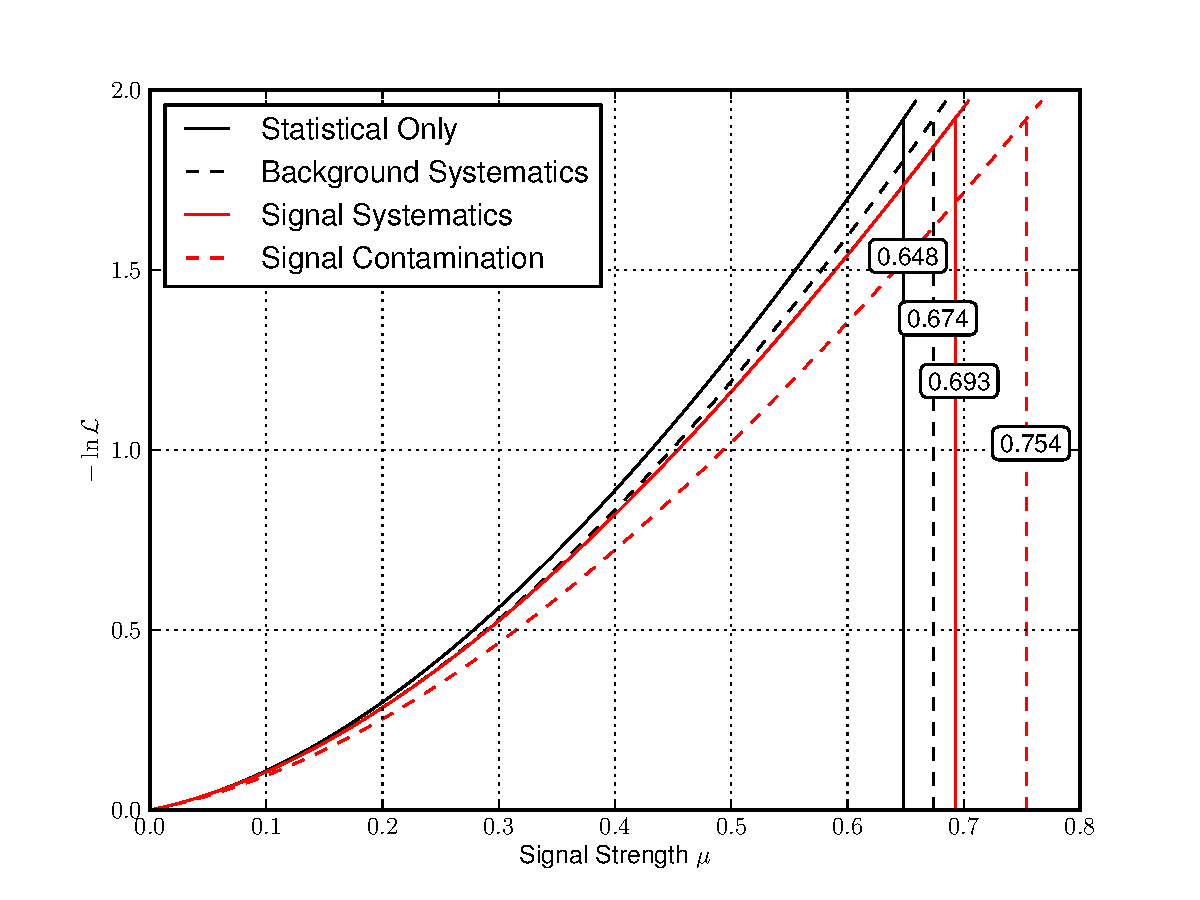
\includegraphics[width=0.47\textwidth]{fig/pl_systematics_80_400}}\quad
\subfloat[Muon channel only]{\label{fig:inter_pl_80_400_muon}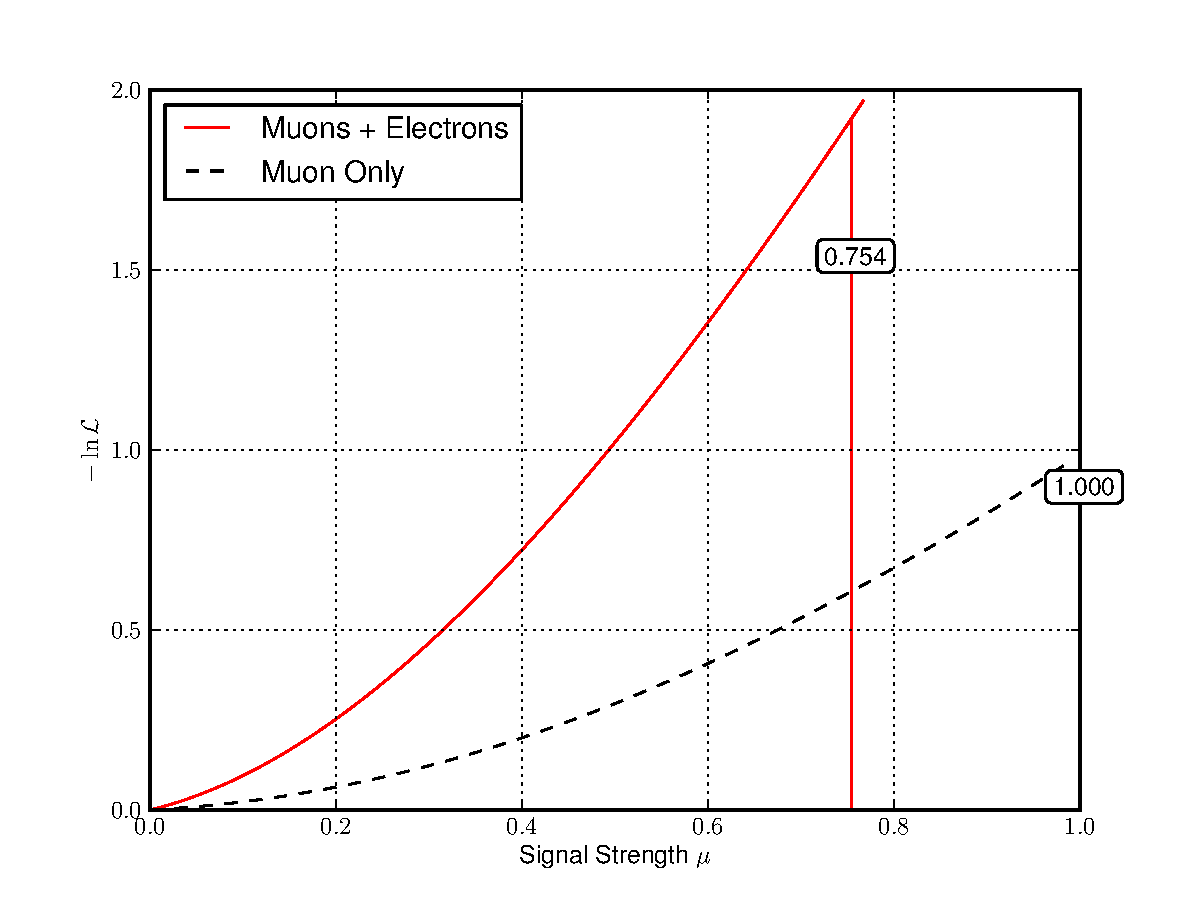
\includegraphics[width=0.47\textwidth]{fig/pl_muon_80_400}}
\caption[The profile likelihood as a function of $\mu$]{The profile likelihood
  as a function of $\mu$ \subref{fig:inter_pl_80_400_syst} with different
  systematic effects included in the likelihood and
  \subref{fig:inter_pl_80_400_muon} with the electron channel removed. The results
  are shown for the \ac{CMSSM} point $(\Mzero, \Mhalf) = (80, 400)$. }
\label{fig:inter_pl}
\end{figure}

\begin{figure}[h!]
\centering
\subfloat[Statistical Unc.]{
  \label{fig:inter_cls_80_400_syst1}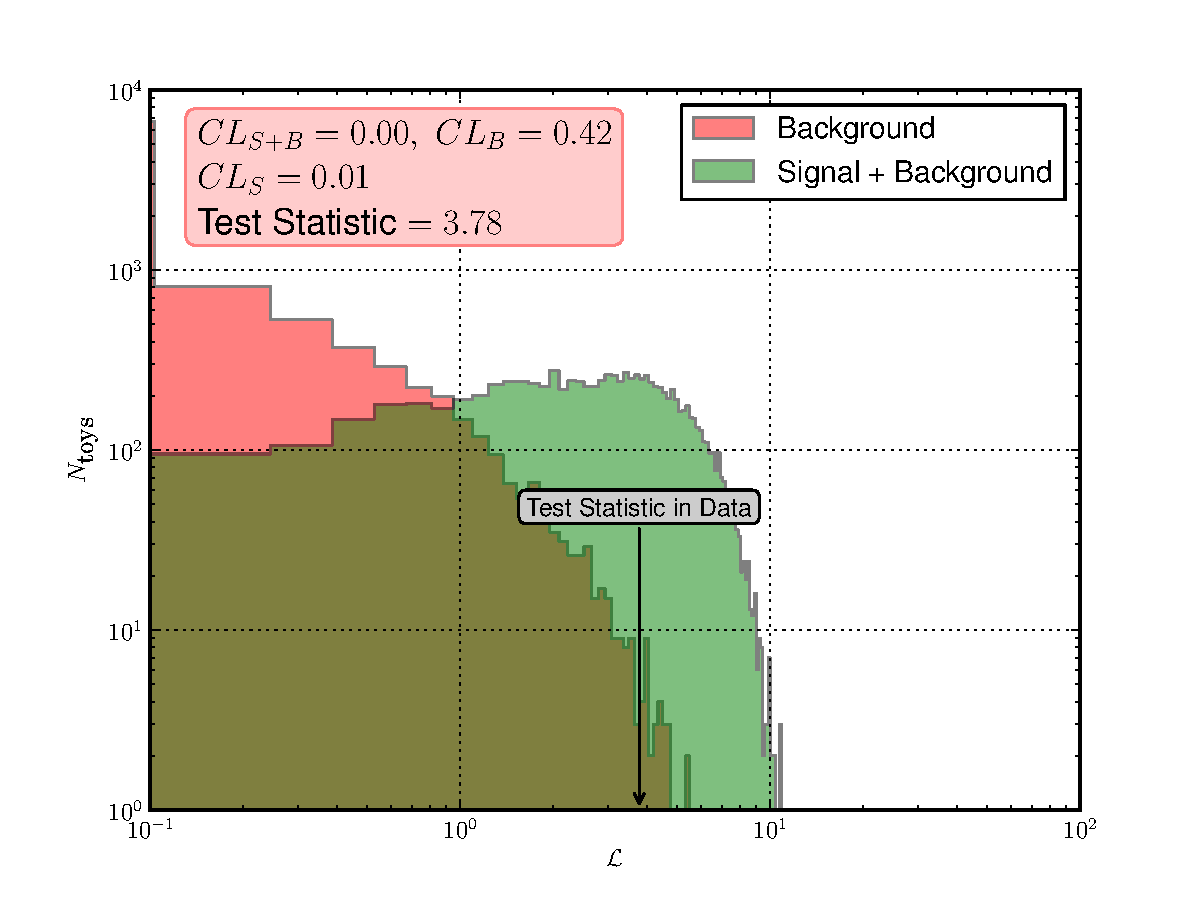
\includegraphics[width=0.32\textwidth]{fig/exp_muon_electron_80_400_bgsysts_no_sigsysts_no_sigcon_no}}
\subfloat[Background Unc.]{
  \label{fig:inter_cls_80_400_syst2}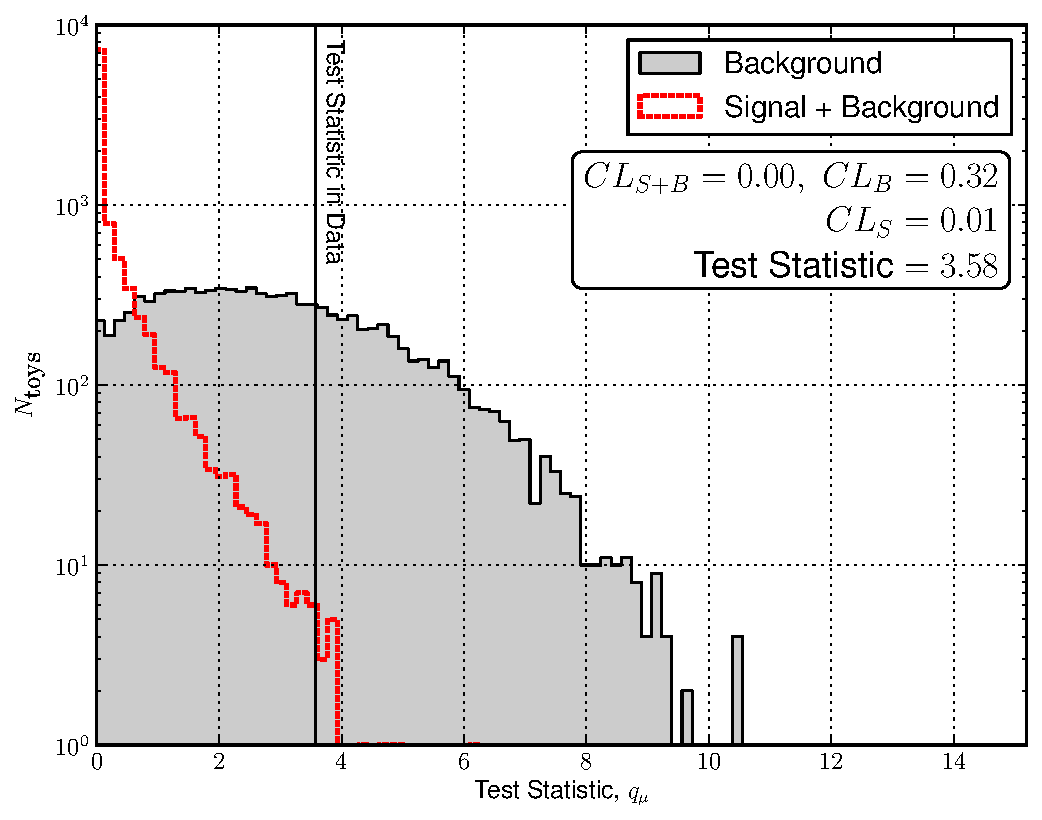
\includegraphics[width=0.32\textwidth]{fig/exp_muon_electron_80_400_bgsysts_yes_sigsysts_no_sigcon_no}}
\subfloat[Signal Unc.]{
  \label{fig:inter_cls_80_400_syst3}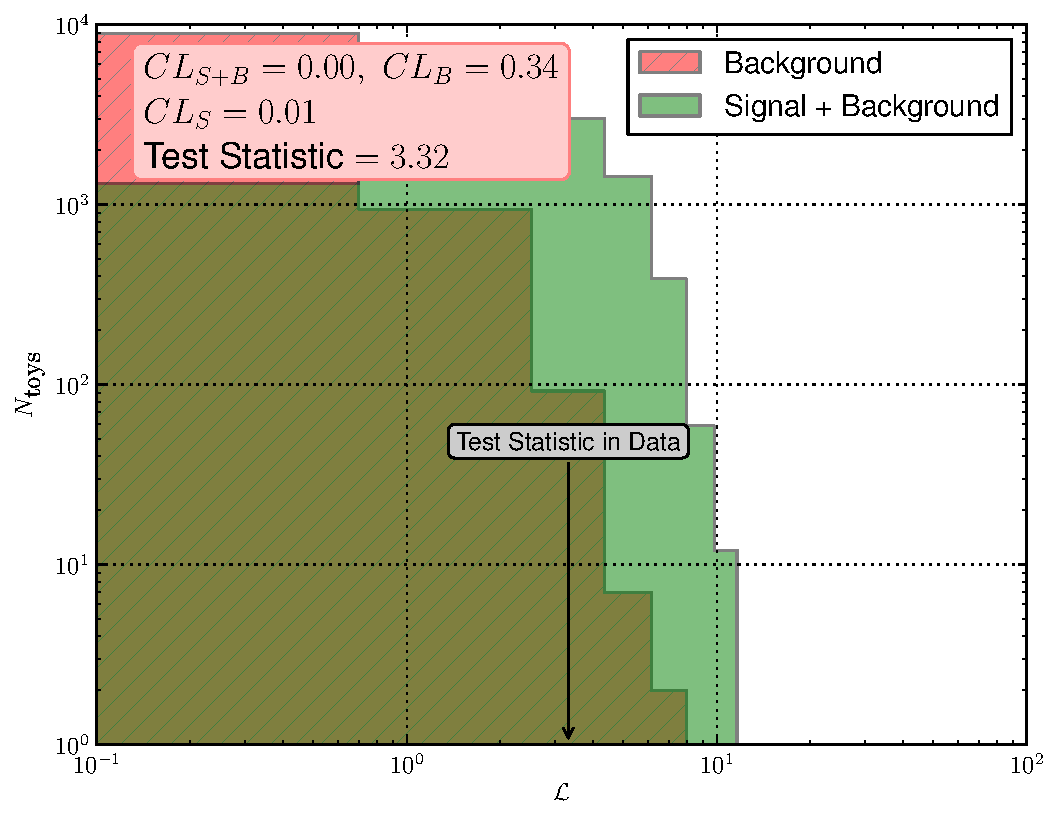
\includegraphics[width=0.32\textwidth]{fig/exp_muon_electron_80_400_bgsysts_yes_sigsysts_yes_sigcon_no}}\\
\subfloat[Signal Contamination]{
  \label{fig:inter_cls_80_400_syst4}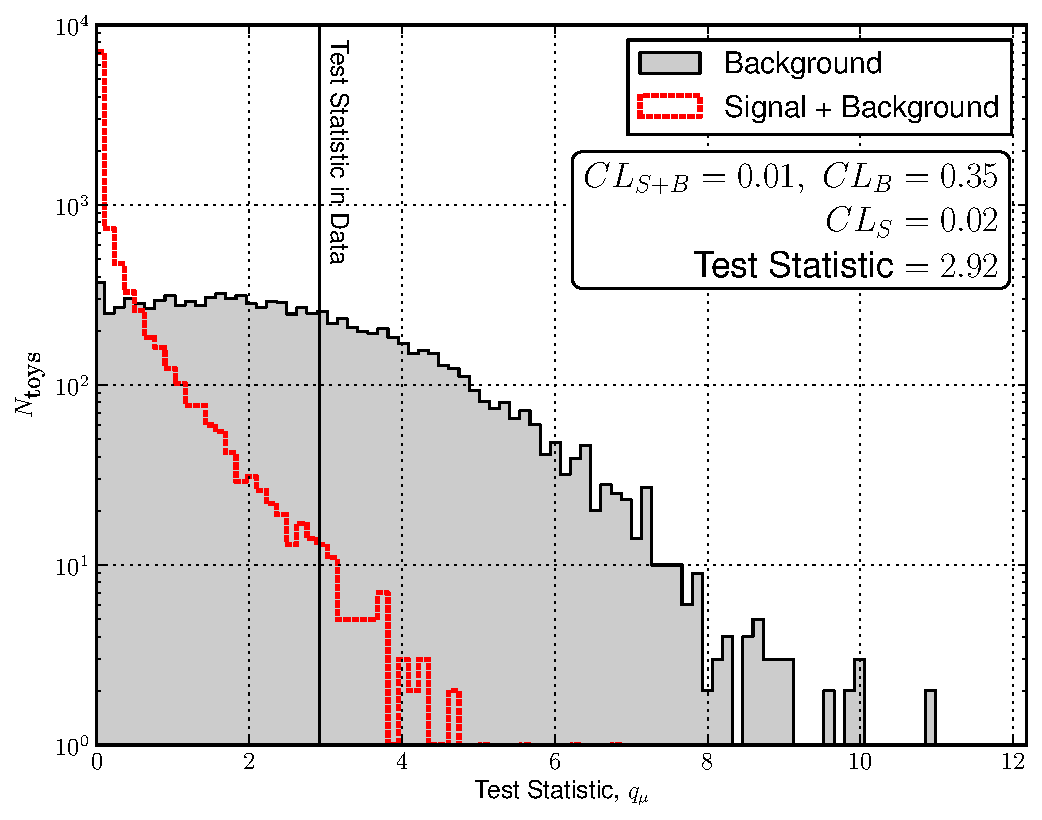
\includegraphics[width=0.32\textwidth]{fig/exp_muon_electron_80_400_bgsysts_yes_sigsysts_yes_sigcon_yes}}
\subfloat[Muon Channel Only]{
  \label{fig:inter_cls_80_400_muon}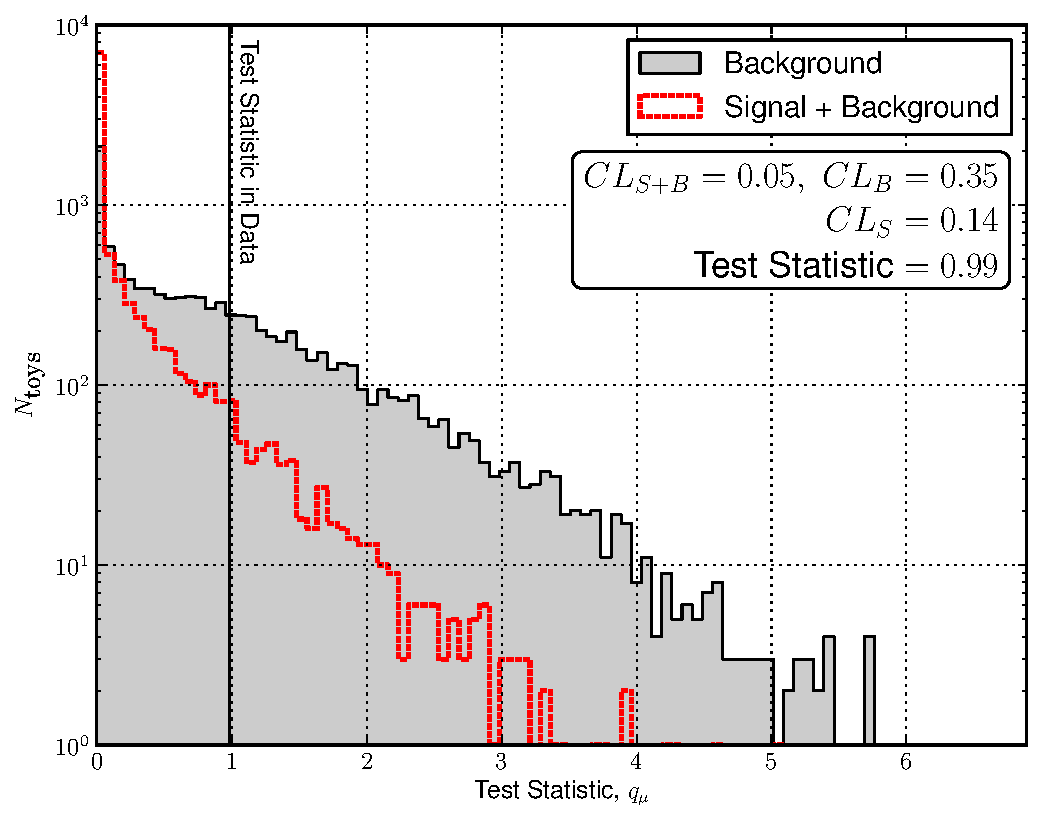
\includegraphics[width=0.32\textwidth]{fig/exp_muon_80_400_bgsysts_yes_sigsysts_yes_sigcon_yes}}
\caption[Distributions of the test statistic, $q_{\mu}$]{Distribution of the
  test statistic, $q_{\mu}$, for null and alternate hypotheses with different
  systematic effects included and with the electron channel removed. These
  distributions have been made for the \ac{CMSSM} point $(\Mzero, \Mhalf) = (80,
  400)$. The values of \CLb, \CLspb and \CLs are also shown.}
\label{fig:inter_cls}
\end{figure}

\subsection{Validation}
\label{sec:inter_validation}
To validate the model, a number of cross-checks are performed. Firstly, the
\ac{PL} and \CLs methods are compared and found to agree. In general, the \CLs
method is expected to be more conservative by covering the full range of the
nuisance parameters in the model.

To see how the \ac{PL} and \CLs results change with modifications to the
likelihood function, a representative point in the \ac{CMSSM} plane
($\tan\beta=10$, $A_0=0$, $\mu>0$) has been chosen. This is $(m_0,
m_{\frac{1}{2}}) = (80, 400)$ - close to the edge of the region excluded by the
data (additional detail can be found in
Appendix~\ref{sec:app_inter_validation}).

The form of the \ac{PL} function for the same point can be seen in
\fig~\ref{fig:inter_pl}. The signal strength, $\mu$, is the ratio of the
excluded cross-section to that predicted by the \ac{CMSSM}. As expected, the
inclusion of systematic effects pushes the exclusion to larger values of
$\mu$. A similar, but more pronounced, effect can be seen when removing the
electron channel. This shows, qualitatively at least, that the model is behaving
as expected. For this particular model point, the signal contamination appears
to have the largest effect, followed by the background uncertainties and then
the signal uncertainties. Note that certain uncertainties are included in all
cases: the effect of the statistical uncertainty in the control region, and the
luminosity uncertainty. The former is actually the dominant uncertainty on the
background prediction. This perhaps explains why the addition of the other
systematic uncertainties appears to have relatively little effect.

The distributions of the test statistic used to calculate \CLs are shown in
\fig~\ref{fig:inter_cls}. The results are seen to be qualitatively similar to
the \ac{PL} case. This particular point goes from being strongly excluded at $>
95\%$ confidence level with both lepton channels, to not being excluded when the
electrons are removed.

\section{Results}
The statistical machinery described so far has been used to give interpretations
in the context of several \ac{NP} models. First of all, the \ac{CMSSM}, and
subsequently two simplified models: \Ttwott and \TthreeW. These are fully
described in \sec~\ref{sec:framework_susy}.

\begin{figure}[h!]
\centering
\subfloat[$250 < \STlep < 350$]{\label{fig:inter_msugra_mu_eff250}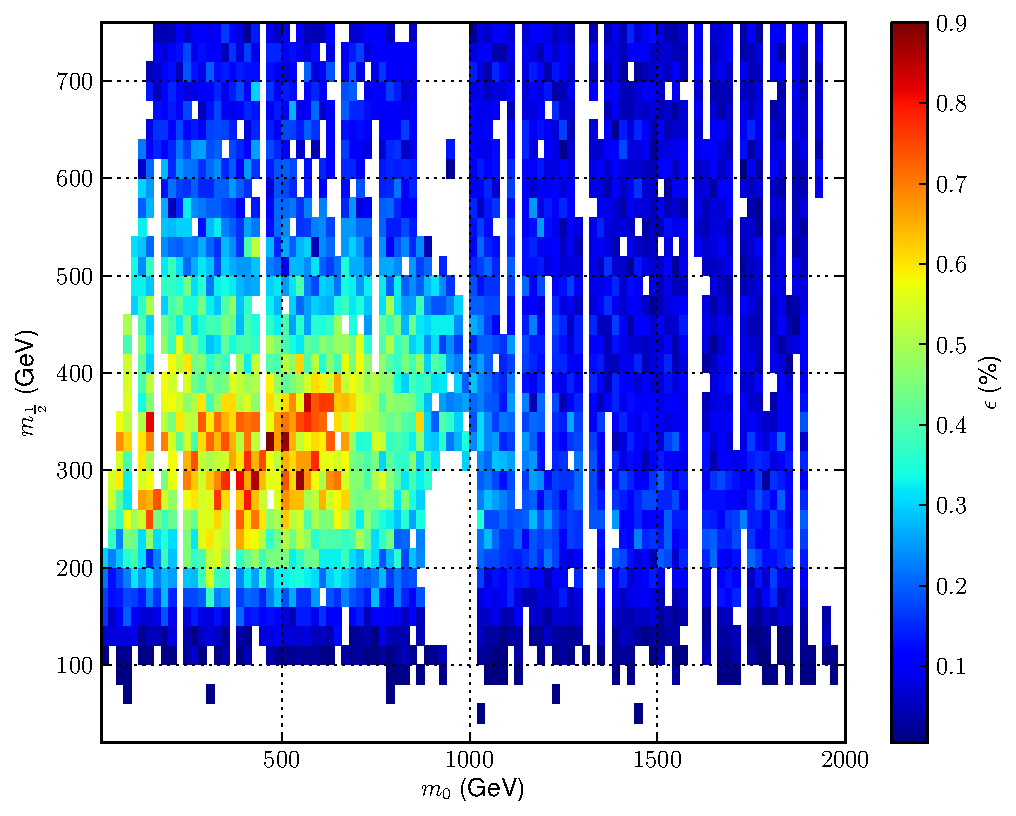
\includegraphics[width=0.49\textwidth]{fig/msugra_muons_eff_250}}
\subfloat[$350 < \STlep < 450$]{\label{fig:inter_msugra_mu_eff350}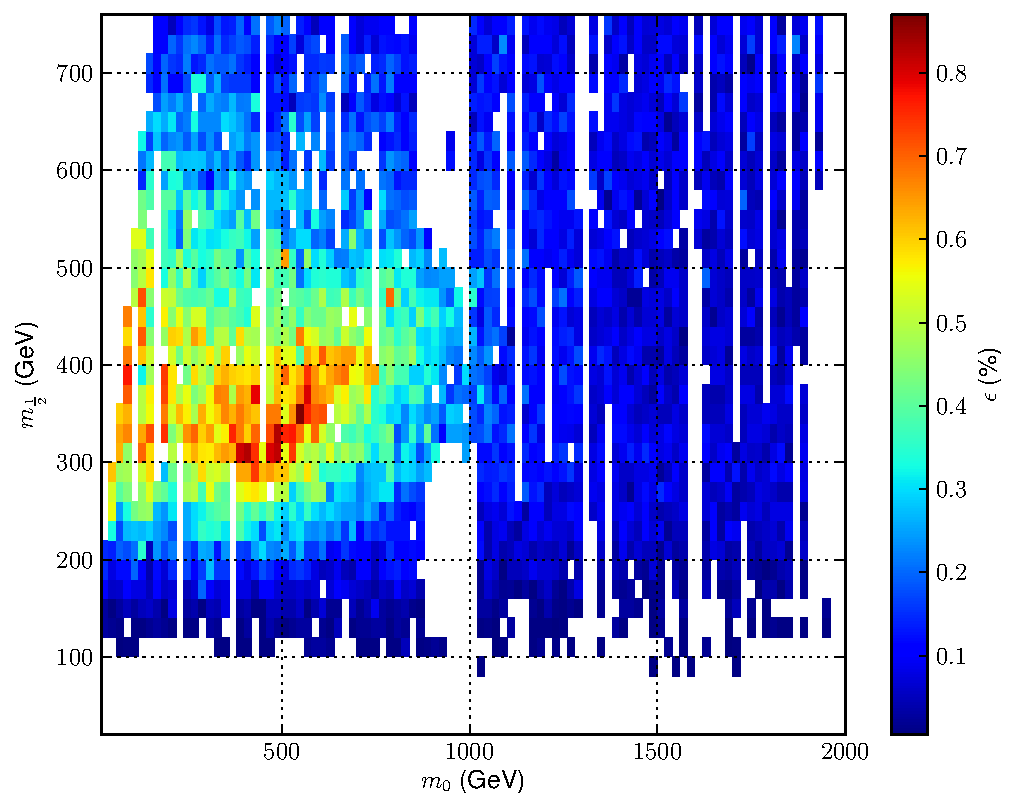
\includegraphics[width=0.49\textwidth]{fig/msugra_muons_eff_350}}\\
\subfloat[$\STlep > 450$]{\label{fig:inter_msugra_mu_eff450}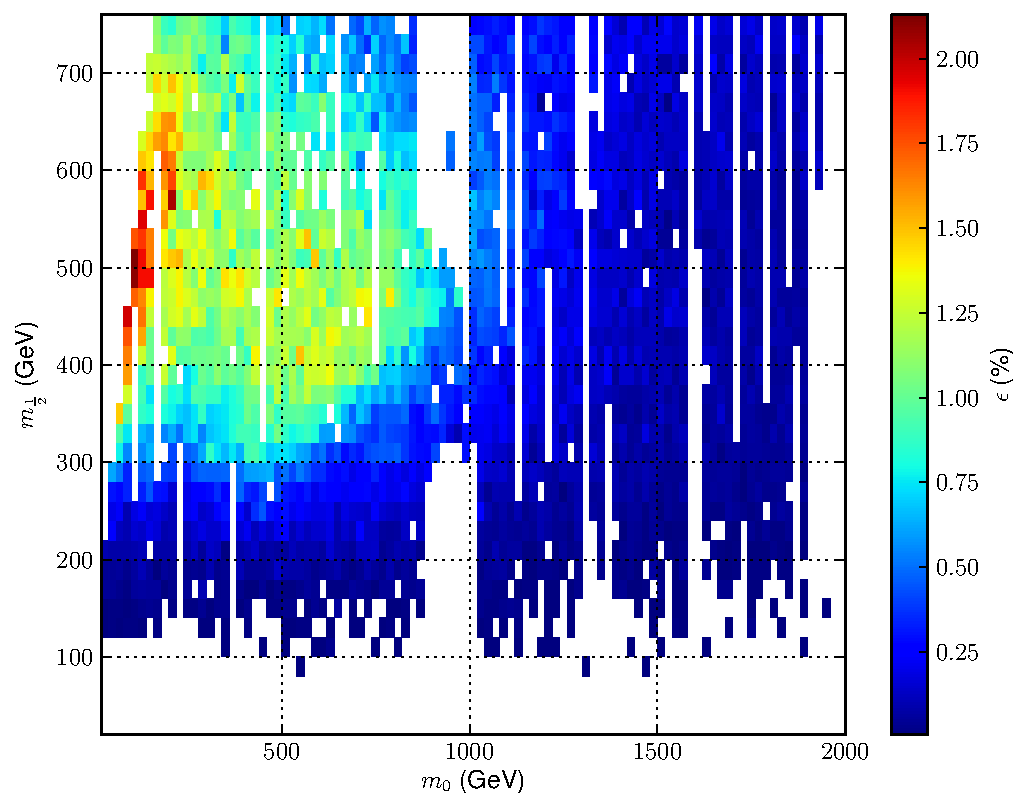
\includegraphics[width=0.49\textwidth]{fig/msugra_muons_eff_450}}
\subfloat[Total]{\label{fig:inter_msugra_mu_efftot}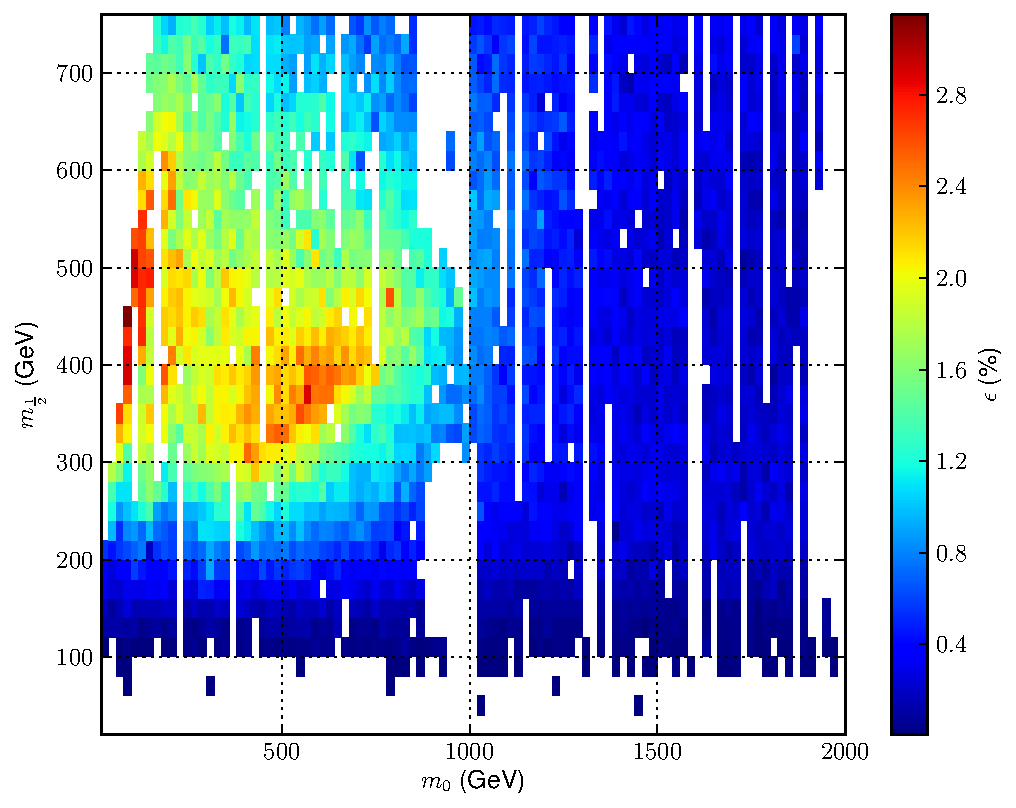
\includegraphics[width=0.49\textwidth]{fig/msugra_muons_eff_total}}
\caption[Signal efficiency for the muon channel in the \ac{CMSSM}]{Signal
  efficiency for the muon channel in the \ac{CMSSM}. The efficiency is shown
  separately for each \STlep bin and as a total. The efficiency is shown in the
  $(\Mzero, \Mhalf)$ plane with $\tanbeta=10$, $\Azero=0$ and $\mu > 0$.}
\label{fig:inter_msugra_mu}
\end{figure}

\begin{figure}[h!]
\centering
\subfloat[$250 < \STlep < 350$]{\label{fig:inter_msugra_el_eff250}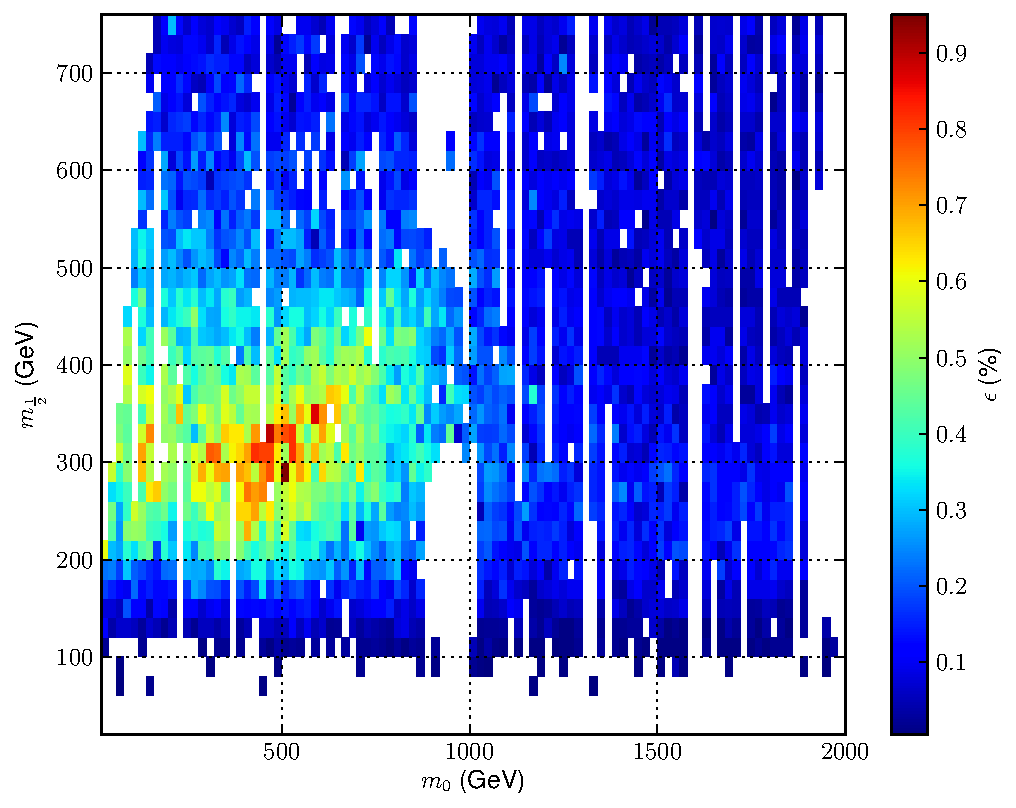
\includegraphics[width=0.49\textwidth]{fig/msugra_electrons_eff_250}}
\subfloat[$350 < \STlep < 450$]{\label{fig:inter_msugra_el_eff350}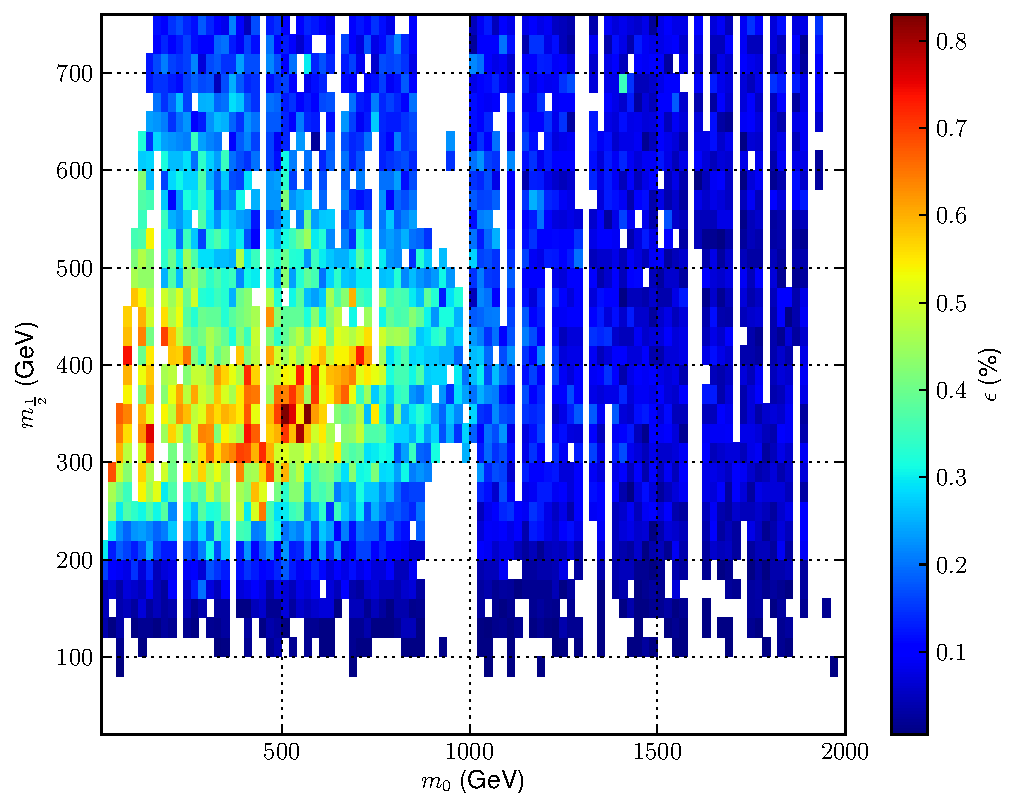
\includegraphics[width=0.49\textwidth]{fig/msugra_electrons_eff_350}}\\
\subfloat[$\STlep > 450$]{\label{fig:inter_msugra_el_eff450}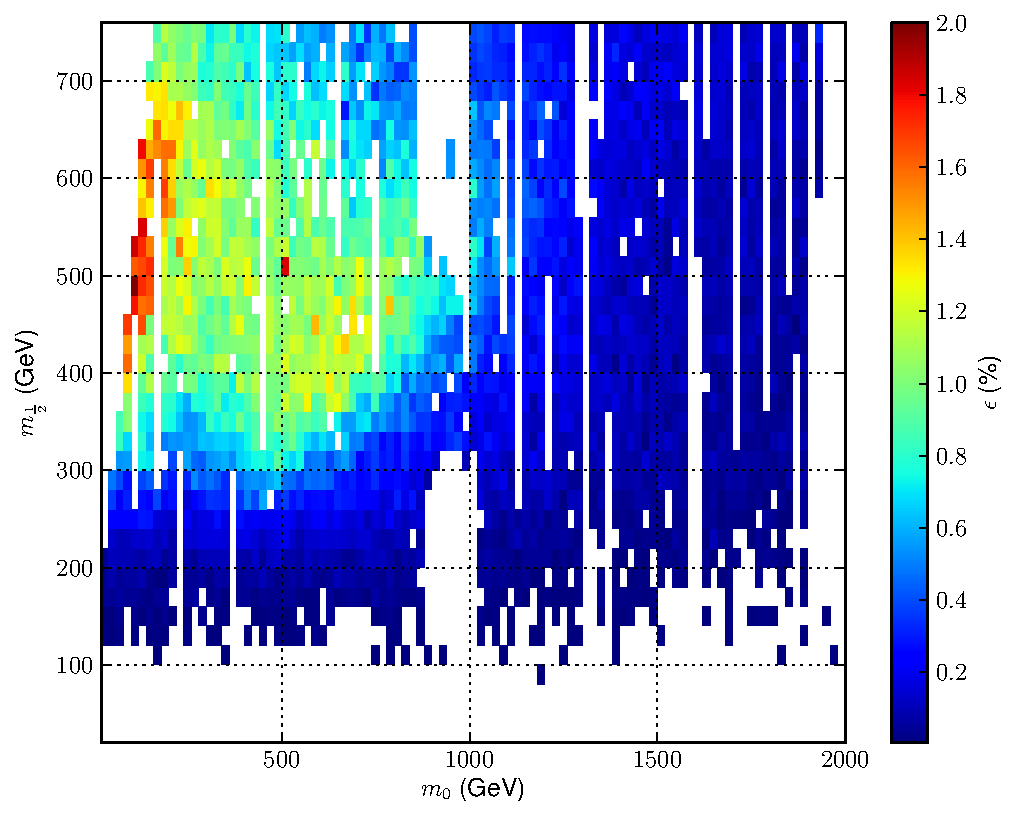
\includegraphics[width=0.49\textwidth]{fig/msugra_electrons_eff_450}}
\subfloat[Total]{\label{fig:inter_msugra_el_efftot}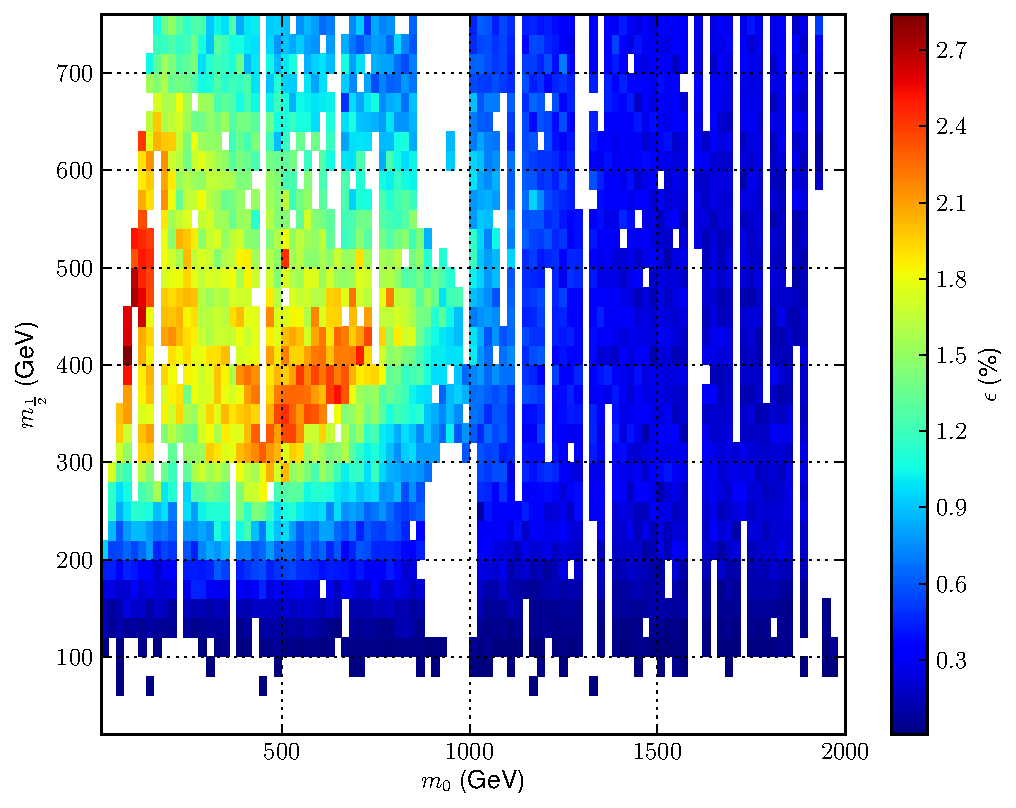
\includegraphics[width=0.49\textwidth]{fig/msugra_electrons_eff_total}}
\caption[Signal efficiency for the electron channel in the \ac{CMSSM}]{Signal
  efficiency for the electron channel in the \ac{CMSSM}. The efficiency is shown
  separately for each \STlep bin and as a total. The efficiency is shown in the
  $(\Mzero, \Mhalf)$ plane with $\tanbeta=10$, $\Azero=0$ and $\mu > 0$.}
\label{fig:inter_msugra_el}
\end{figure}

\begin{figure}[h!]
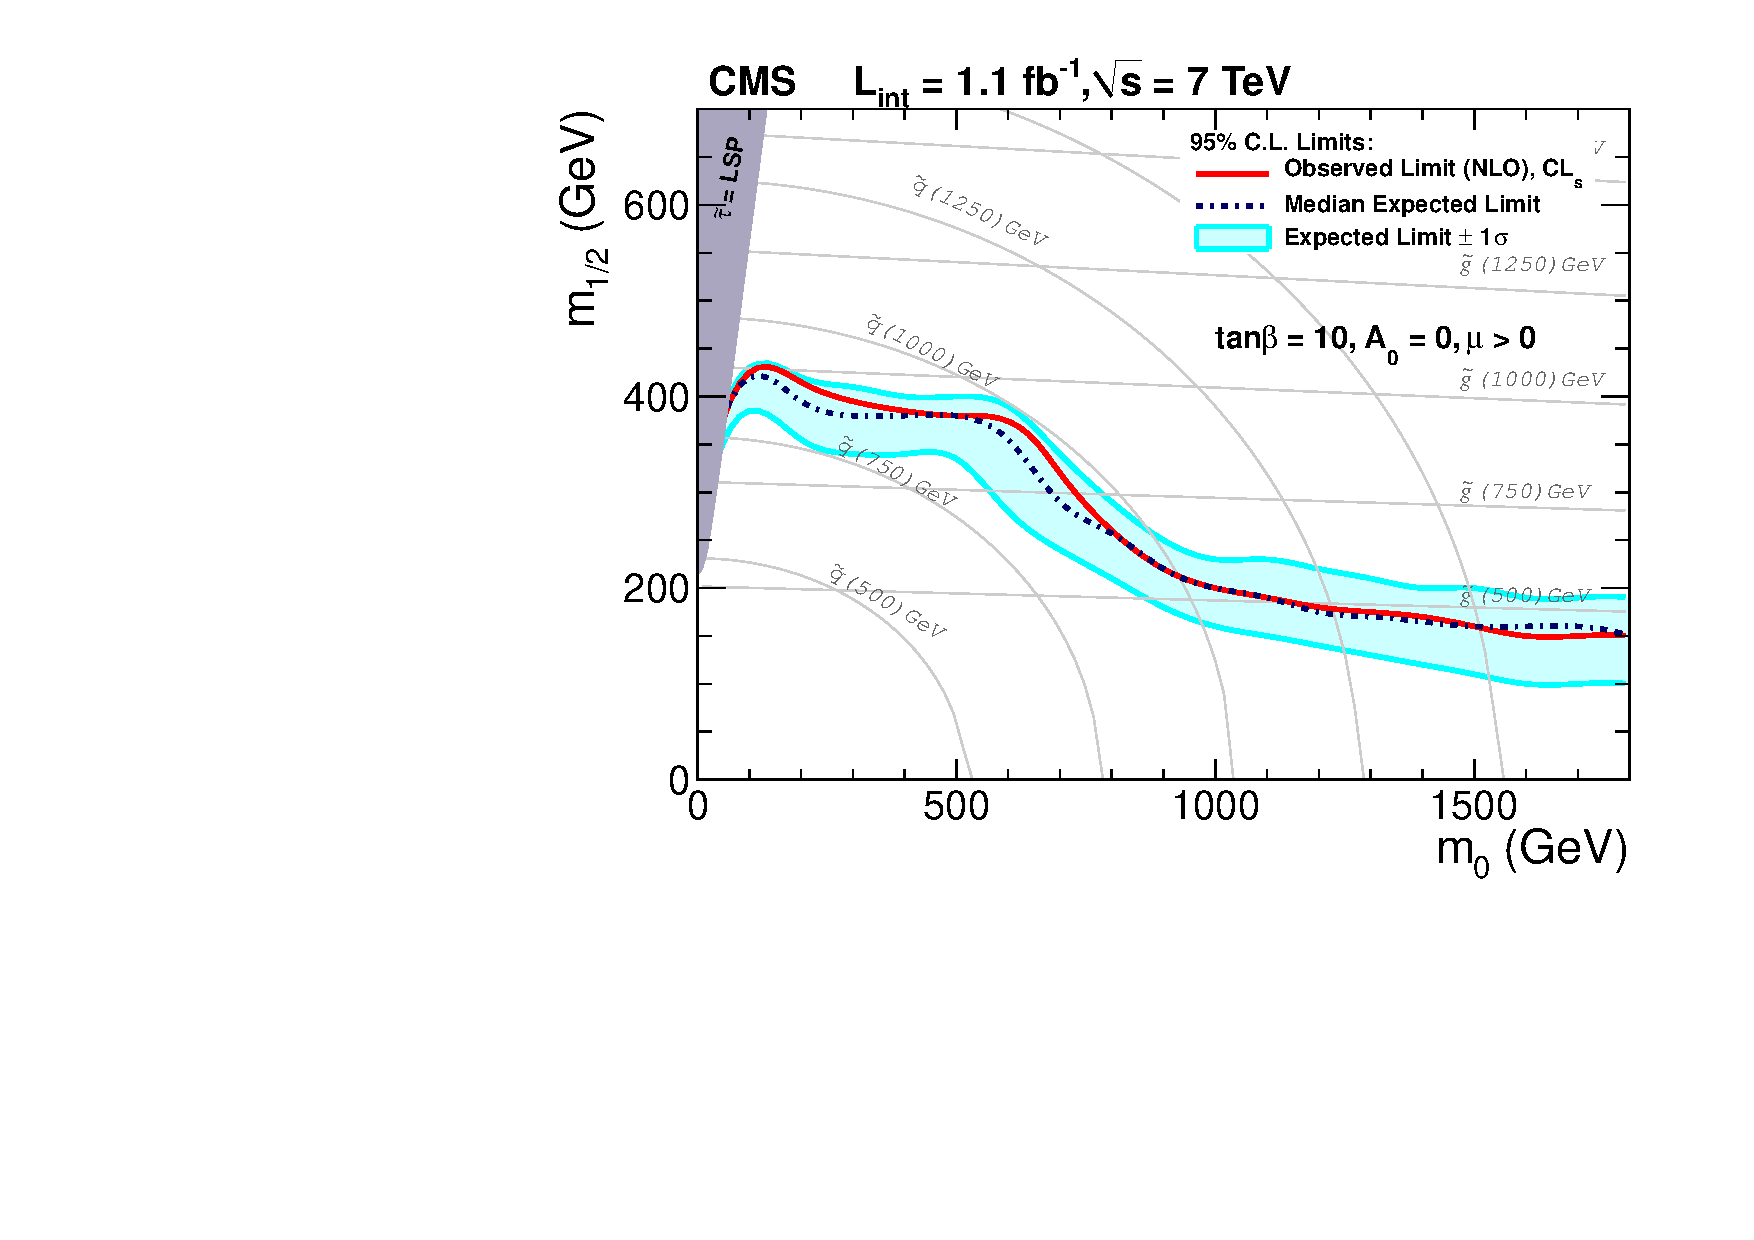
\includegraphics[width=\textwidth]{fig/RA4_ExclusionLimit_tanb10}
\caption[95\% confidence level exclusion plot for the \ac{CMSSM}]{95\%
  confidence level exclusion plot for the \ac{CMSSM}. The observed (red),
  expected (blue dotted) and $\pm 1\sigma$ exclusion bands (light blue shaded)
  are shown. These are calculated using the \CLs method. Lines of constant
  squark and gluino mass are also shown.}
\label{fig:inter_msugra_exclusion}
\end{figure}

\subsection{The \ac{CMSSM}}
The \ac{CMSSM} was previously described in \sec~\ref{sec:cmssm}. As explained,
the \ac{CMSSM} makes a number of somewhat arbitrary choices which restrict the
\ac{SUSY} toplogies signatures it is able to encompass. Whilst these make it
relatively undesirable as a framework for theoretical interpretation, it is
nonetheless useful as a common yardstick by which to compare experiments and
searches.

The \ac{CMSSM} results are presented as a 95\% exclusion in a two-dimensional
plane of the parameter space where the two mass parameters, \Mzero and \Mhalf,
are allowed to vary. Other parameters are fixed as follows: $\Azero = 0$,
$\tanbeta = 10$ and $\mu > 0$.

\subsubsection{Technical Details}
The likelihood function detailed in \sec~\ref{sec:inter_1lepton} takes as input
the signal efficiencies for each bin of \STlep. In the case of the \ac{CMSSM},
these must be evaluated for each point in the $(\Mzero, \Mhalf)$-plane. These
are evaluated using the same analysis procedure as used for the data and \ac{SM}
\ac{MC} samples. The \ac{CMSSM} sample is produced using the Pythia event
generator, with the two mass parameters are varied independently in steps of
\unit{20}{\GeV} to produce a grid. For each grid point, 10000 events are
generated. Due to the large number of events, the detector response is simulated
using the \fastsim simulation package (see \sec~\ref{sec:cms_computing}). This
has been extensively validated and tuned against the full detector simulation
and shown to give adequate results for many analyses.

Having evaluated the efficiencies per \STlep bin for each \ac{CMSSM} grid point,
the \ac{NLO} cross-sections are calculated using the \prospino
package~\cite{prospino}. The cross-sections are calculated individually for each
\ac{SUSY} subprocess and then combined according to the composition of the
analysis selection. These are then input to the limit code, along with the
required uncertainties and model-independent parameters.

\subsubsection{Efficiencies}
The efficiency per \STlep bin of the analysis selection as a function of the
\ac{CMSSM} parameter space is shown in \figs~\ref{fig:inter_msugra_mu} and
\ref{fig:inter_msugra_el} for muons and electrons respectively. The ``holes'' in
the \ac{CMSSM} sample are due to incomplete data samples at the time of
publication.

The efficiencies give a good indication of the sensitivity of the analysis to
different regions of the parameter space. Firstly, it can be seen that
regardless of the \STlep bin, significant efficiency is achieved only for values
of $\Mzero < \unit{1000}{\GeV}$. The correlation of \STlep and \Mhalf should
also be noted - with the higher bins generally sensitive to larger values of
\Mhalf. Since \STlep is sensitive to the mass of the \ac{LSP} which increases
linearly with \Mhalf and is insensitive to to \Mzero (see~\cite{sparticles}
p290), this would appear to be consistent.

\subsubsection{Exclusion}
For consistency with other \ac{SUSY} searches at the \ac{LHC}, a limit has been
set using the \CLs method described in \sec~\ref{sec:inter_cls}. Whilst it is
possible, to set an upper limit on the signal strength parameter, $\mu$, this
becomes highly computationally intensive. Instead, a simple exclusion is
produced assuming \ac{NLO} cross-sections. This is shown in
\fig~\ref{fig:inter_msugra_exclusion}. All terms discussed in
Appendix~\ref{sec:inter_1lepton} have been included. The expected limit and $\pm
1\sigma$ bands are evaluated by setting the observations for each bin to be
exactly that predicted from data.

The exclusion seems to be well predicted by the efficiency maps, with
significant exclusion on the \Mhalf axis only at low \Mzero. As can be seen,
squark masses below $\approx \unit{900}{\GeV}$ and gluino masses below $\approx
\unit{500}{\GeV}$ are excluded at 95\% confidence.


\subsection{Simplified Models}
\subsubsection{Technical Details}
The simplified models described in \sec~\ref{sec:sms} are simulated using the
Pythia generator by reusing \ac{SUSY} subprocesses. The mass parameters in each
model are varied in steps. By varying the masses of the squark or gluino,
\ac{LSP} and other intermediate particles, a grid of simplified model points is
created. These are then processed further as for the \ac{CMSSM}.

For the simplified models shown here, the mother and daugther particles masses
(\Mgluino or \Mstop and \Mlsp) are varied in steps of \unit{20}{\GeV}. Since the
mother particle must be at least as massive as the daughter, half of the
parameter space is unphysical and hence excluded.

To provide the most detailed interpretation of the simplified models, it is
desirable to calculate an upper limit on the cross-section for each grid
point. This can be contrasted to the case of the \ac{CMSSM}, where the
cross-section at each point is known and a simple exclusion contour is
sufficient. Due to the comptuational difficulty of calculating a confidence
interval using the \CLs method, the \ac{PL} method has been used instead. In
addition, further simplification of the likelihood is achieved by including a
single nuisance parameter for the signal efficiency uncertainty. This is then
assigned a conservative 25\% uncertainty, constant across the model parameter
space. This value is chosen by taking representative values of the \MET scale
and resolution uncertainties given in Table~\ref{tbl:inter_signal_systematics},
for the \ac{CMSSM}, and adding in quadrature with the 10\% \ac{PDF} uncertainty:
\begin{equation*}
\underbrace{\left(10\%\right)^2}_{\textrm{\ac{PDF}}} +
\underbrace{\left(15\%\right)^2}_{\textrm{\ac{JES}}} +
\underbrace{\left(10\%\right)^2}_{\MET~\textrm{resolution}}
\approx 20\%.
\end{equation*}

For the following limit plots, holes in the sample have been filled by taking
the average observed limit of surrounding points. A similar procedure has also
been used to produce smooth exclusion contours.

\subsubsection{\TthreeW}
For the \TthreeW model, the intermediate mass state in the cascade decay
introduces an additional mass parameter, $m_{\PScharginopm}$. Of course, this
parameter should lie somewhere between the mother and daughter particles'
masses. To study a range of scenarios without having to consider the full
three-dimensional volume of the parameter space, three scenarios are
considered. Choosing values of the intermediate particle mass according to
\begin{equation}
\label{eqn:tthreew_x}
\Mchargino = x \Mgluino + (1-x)\Mlsp,
\end{equation}
limits have been set for 3 values of the parameter $x$ -- 0.25, 0.5 and
0.75. Intuitively, these represent cases where the intermediate particle mass is
closer to the daughter, intermediate between daughter and mother and closer to
the mother respectively.

\fig~\ref{fig:inter_t3w_eff} shows total efficiency as a function of
$(\Mgluino, \Mlsp)$ for each plane in $x$, separated by lepton channel. The
efficiency is seen to decrease as the mother and daugther move closer in
mass. When the mass splitting is small, less energy is available for hadronic
and leptonic activity in the event, and thus the efficiency of the analysis cuts
is reduced.

\begin{figure}[h!]
\centering
\subfloat[\Pmu, $x=0.25$]{\label{fig:inter_t3w_0p75_mu_efftot}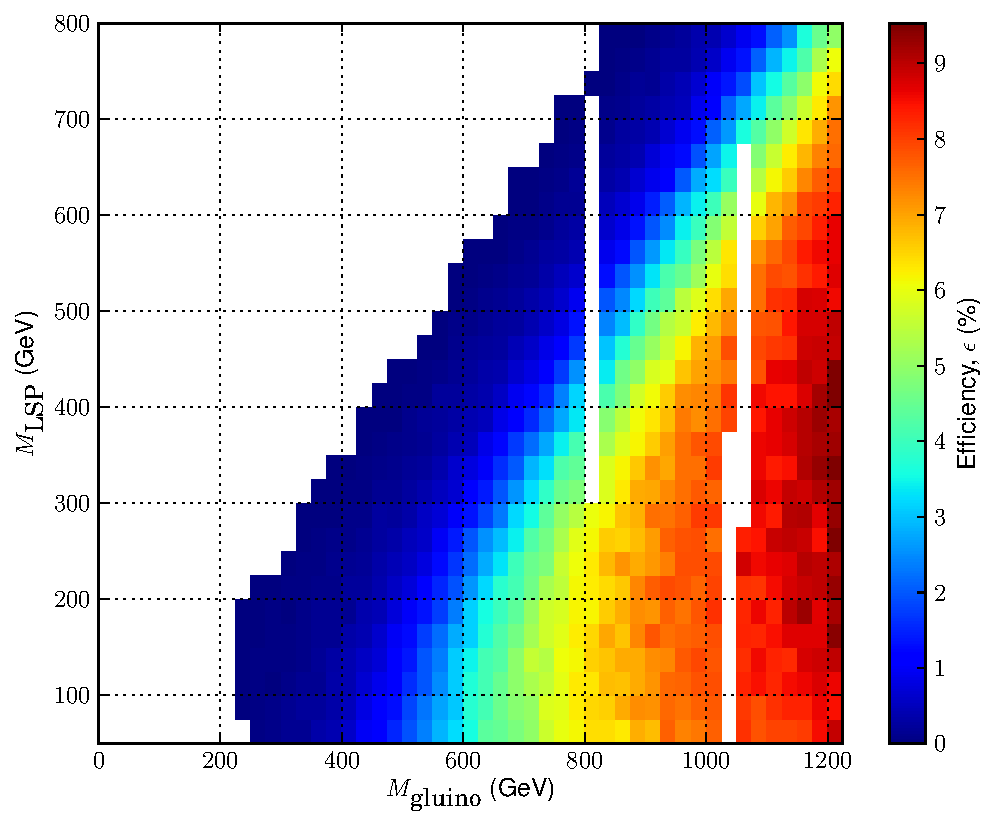
\includegraphics[width=0.43\textwidth]{fig/t3w_0p75_muons_eff_total}}\quad
\subfloat[\Pe, $x=0.25$]{\label{fig:inter_t3w_0p75_el_efftot}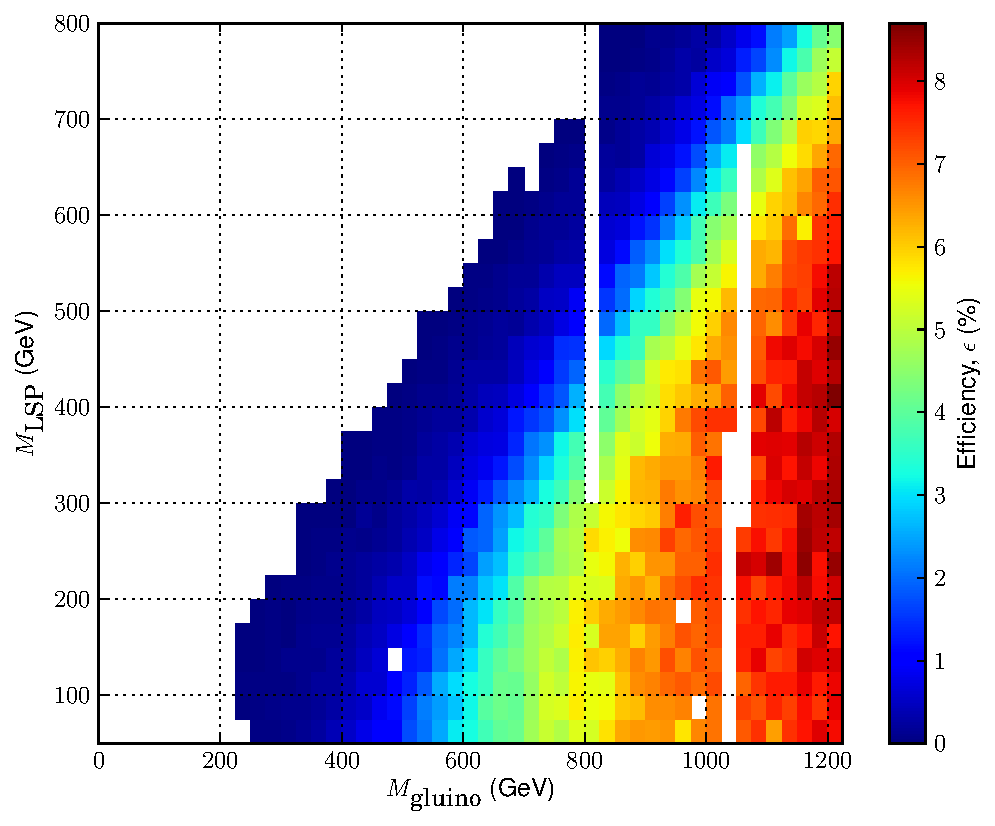
\includegraphics[width=0.43\textwidth]{fig/t3w_0p75_electrons_eff_total}}\\
\subfloat[\Pmu, $x=0.5$]{\label{fig:inter_t3w_0p50_mu_efftot}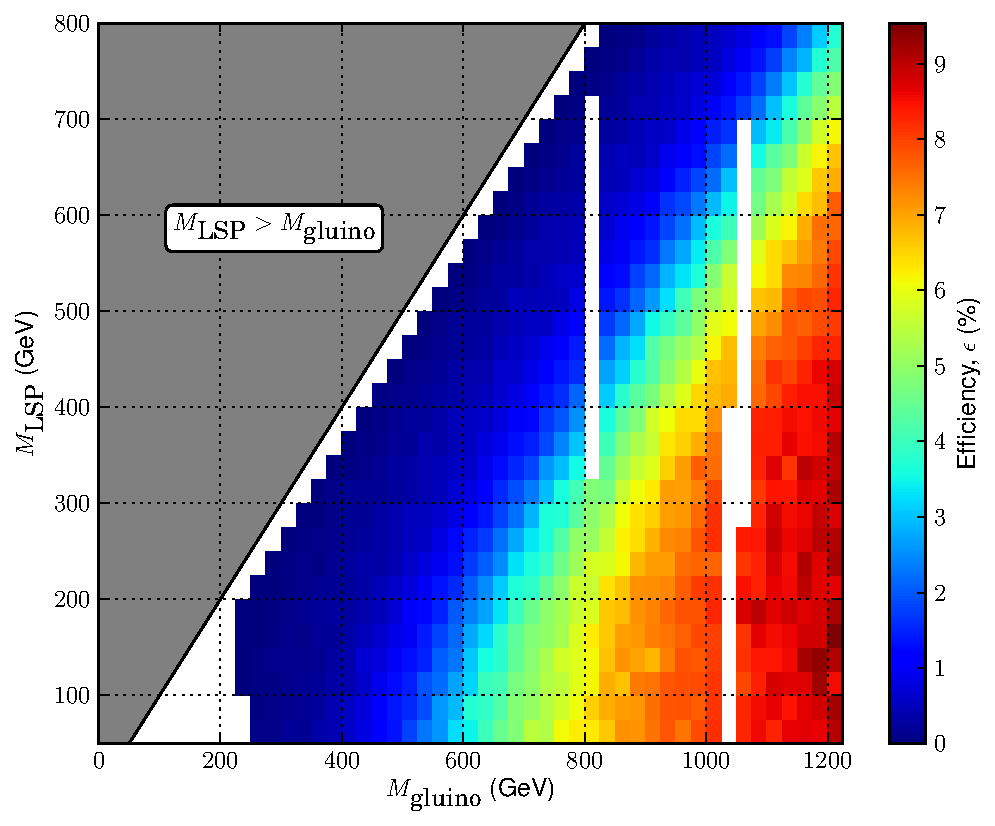
\includegraphics[width=0.43\textwidth]{fig/t3w_0p50_muons_eff_total}}\quad
\subfloat[\Pe, $x=0.5$]{\label{fig:inter_t3w_0p50_el_efftot}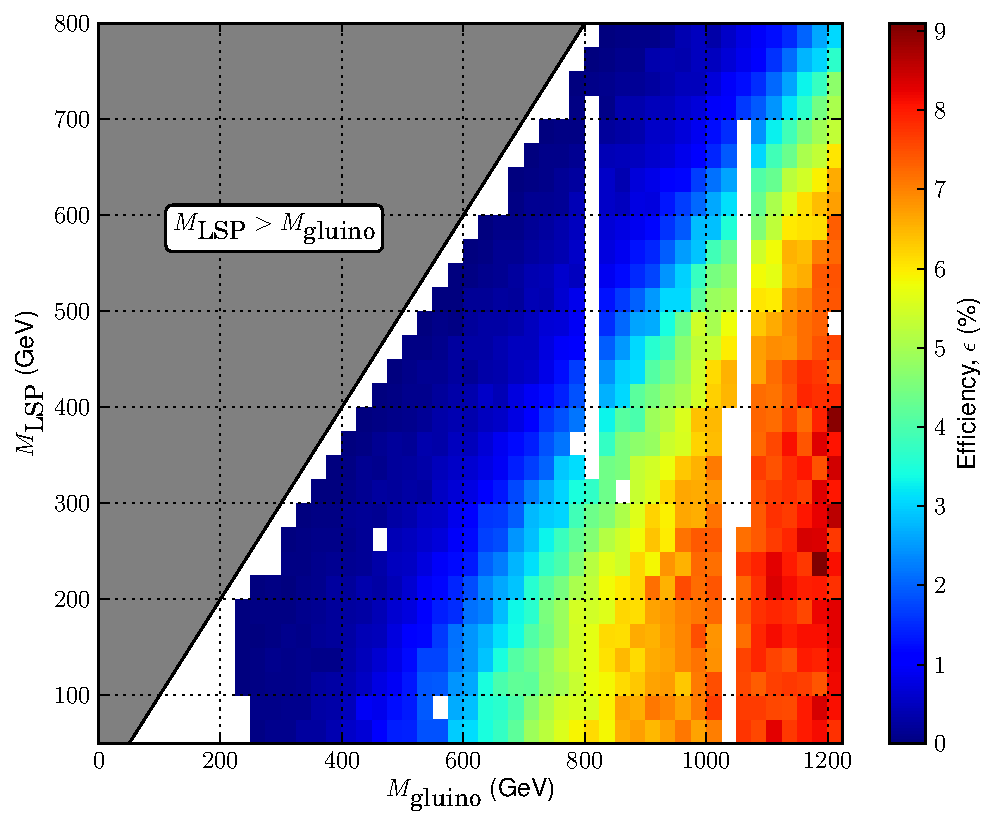
\includegraphics[width=0.43\textwidth]{fig/t3w_0p50_electrons_eff_total}}\\
\subfloat[\Pmu, $x=0.75$]{\label{fig:inter_t3w_0p25_mu_efftot}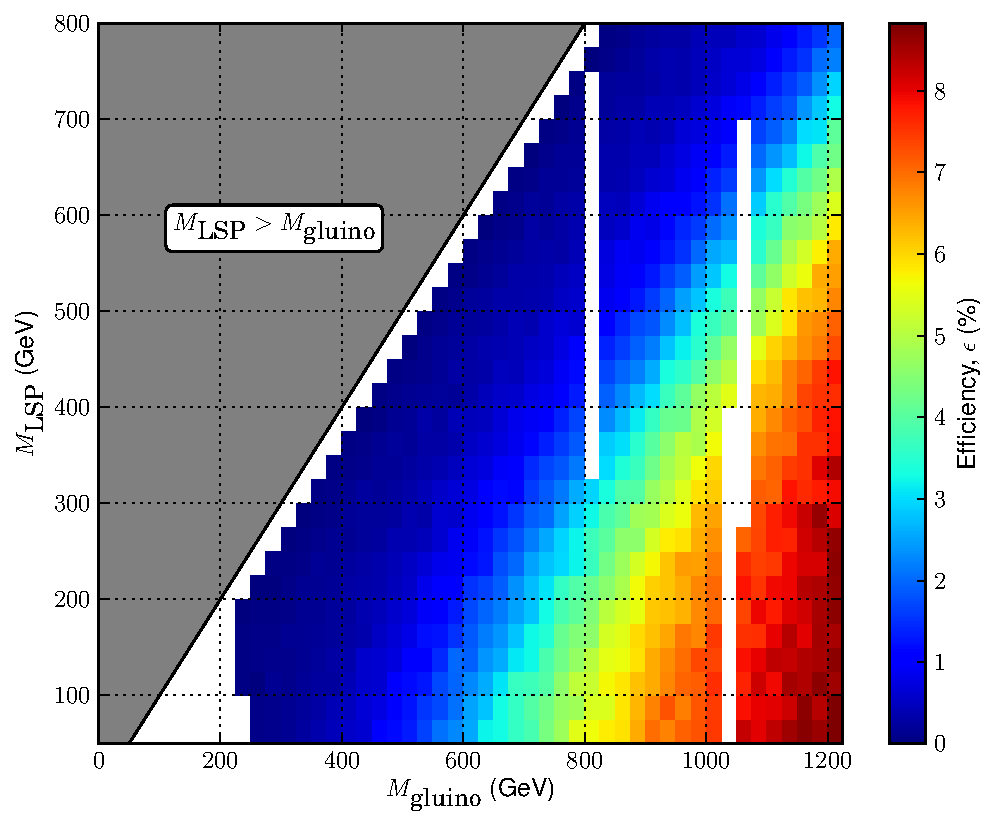
\includegraphics[width=0.43\textwidth]{fig/t3w_0p25_muons_eff_total}}\quad
\subfloat[\Pe, $x=0.75$]{\label{fig:inter_t3w_0p25_el_efftot}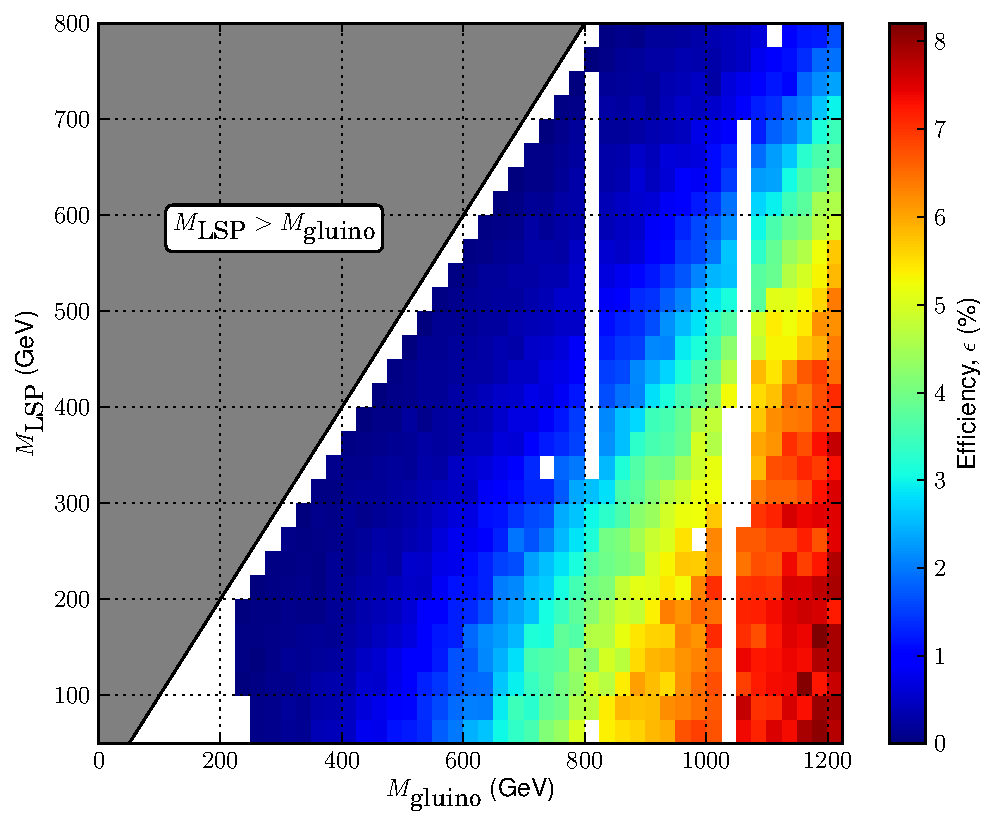
\includegraphics[width=0.43\textwidth]{fig/t3w_0p25_electrons_eff_total}}
\caption[Signal efficiency in the \TthreeW simplified model]{Plots of total
  signal efficiency for muon and electron channels in the \TthreeW simplified
  model. Each plot shows efficiency as a function of $(\Mgluino, \Mlsp)$ for a
  given value of \Mchargino.}
\label{fig:inter_t3w_eff}
\end{figure}

The observed limits for each value of $x$ (0.25, 0.5 and 0.75) are shown in
\figs~\ref{fig:inter_t3w_0p75}, \ref{fig:inter_t3w_0p50} and
\ref{fig:inter_t3w_0p25} respectively. The exclusion contours are compared to a
reference cross-section for squark production calculated using \prospino
assuming \ac{QCD}-strength couplings. For $x=0.25$ and an \ac{LSP} mass of
\unit{200}{\GeV}, gluino masses below \unit{600}{\GeV} are excluded. For
$x=0.5$, the same \ac{LSP} mass yields an exclusion $\Mgluino <
\unit{500}{\GeV}$. For $x=0.75$, the excluded region is $\Mgluino <
\unit{450}{\GeV}$.

For points where $\Mgluino \approx \Mlsp$, there is relatively little energy
available in the cascade. This generally reduces the \HT present in the event,
and consequently the efficiency. Events entering the sample in this region tend
to be dominated by \ac{ISR}. The modelling of \ac{ISR} in simulation has a
significant associated uncertainty. For this reason, the region immediately
below the diagonal has been excluded from the limit. This excluded range is
chosen to remove regions where the upper limit appeared to fluctuate at
random. For $x=0.50$ and $x=0.75$, the region $\Mgluino - \Mlsp <
\unit{100}{\GeV}$ is excluded. For $x=0.25$, \Mchargino is close to \Mlsp and
presumably the efficiency is more sensitive to the modellling of \ac{ISR}. In
this case, the region $\Mgluino - \Mlsp < \unit{140}{\GeV}$ is ignored.

Comparing the exclusion contours, there does not appear to be a strong
dependence on \Mchargino. But the reach of the search can be seen to improve
slightly for lower values of $x$, when the mass splitting between the mother and
the \ac{LSP} is reasonably large. From \eqn~\ref{eqn:tthreew_x}, these models
have an intermediate particle with a mass closer to the \ac{LSP} than to the
mother. In such events, the \PW would be expected to be relatively soft and the
jets from the cascade hard. With respect to the analysis selection, the
efficiency of the \HT cut would be expected to increase. On the other hand, for
a softer \PW, the \STlep efficiency may decrease due to the lower charged lepton
momentum. Overall, the second effect is likely to be small since \STlep is
likely to be dominated by the missing energy from the \acp{LSP}.

In the cases where the mass splitting between mother and \ac{LSP} is smaller,
models with \Mchargino close to \Mgluino appears to give better exclusion. In
these cases, one might guess that the harder \PW is more relevant has a greater
effect on the efficiency since there is less hadronic energy available from the
cascade.

\begin{figure}[h!]
\centering
\subfloat[]{\label{fig:inter_t3w_0p75_limit}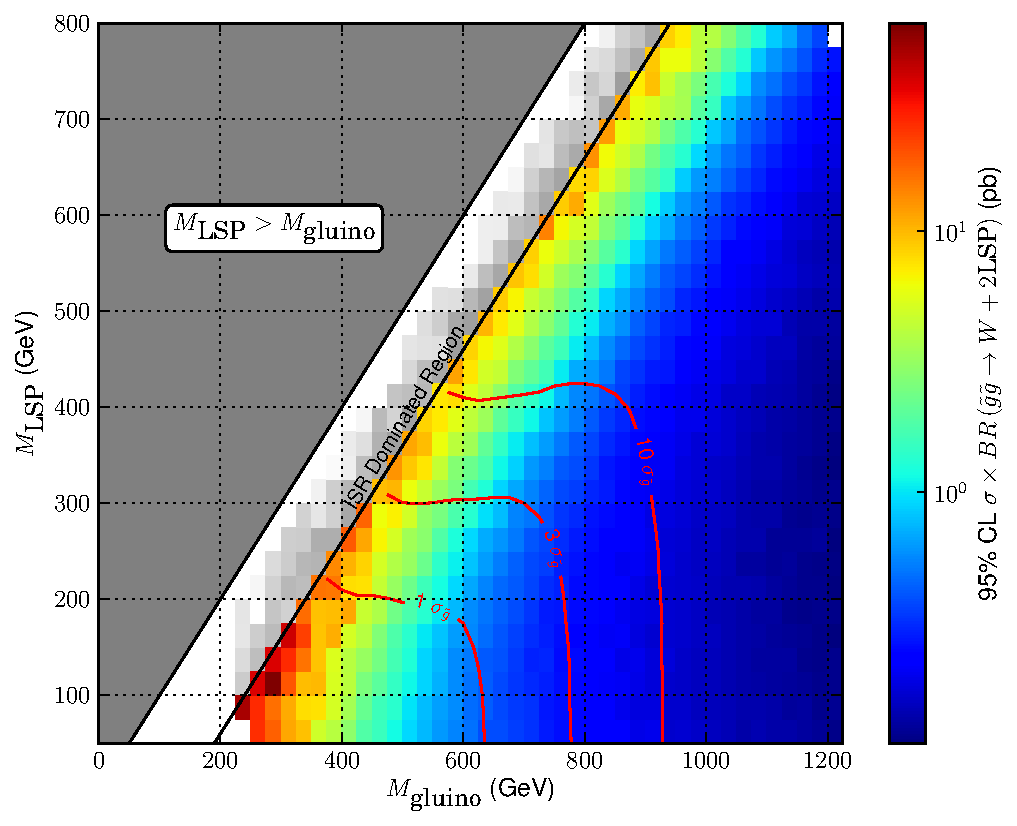
\includegraphics[width=0.49\textwidth]{fig/t3w_0p75_limit_sigsyst}}
\subfloat[]{\label{fig:inter_t3w_0p75_limit_1d}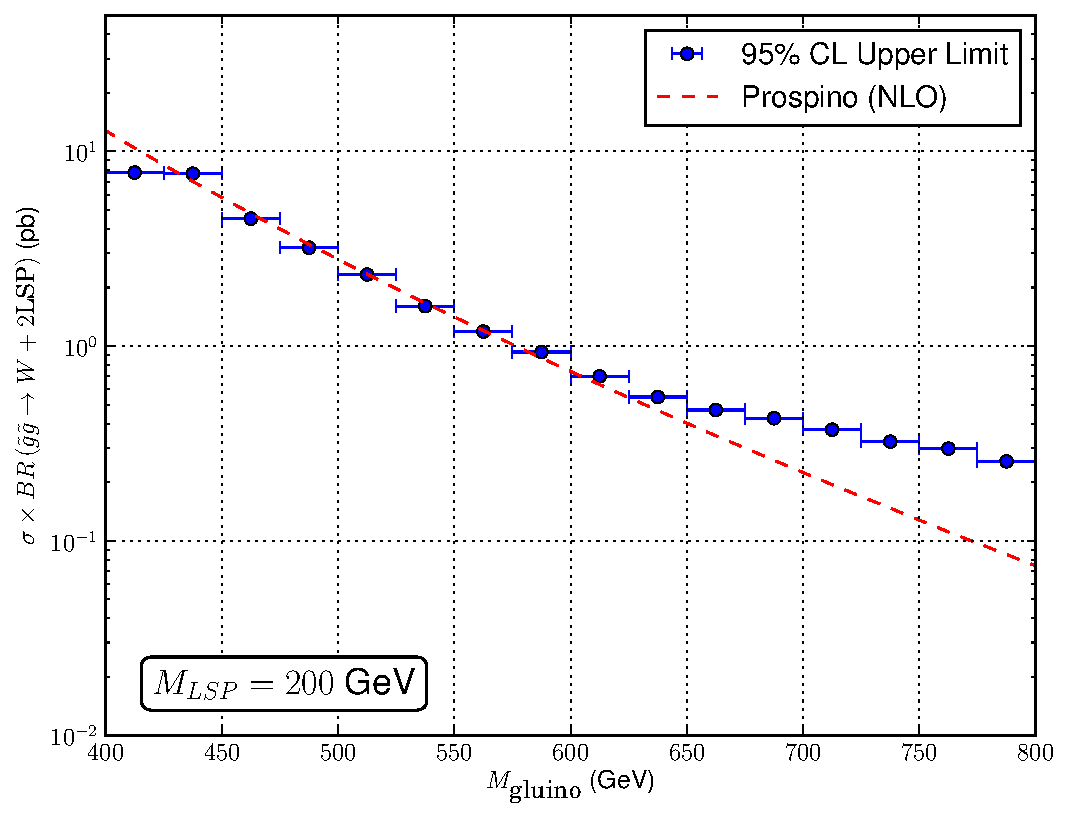
\includegraphics[width=0.49\textwidth]{fig/t3w_0p75_limit_sigsyst_1d}}
\caption[Limit in the \TthreeW simplified model with \Mchargino set assuming
$x=0.25$]{Limit in the \TthreeW simplified model with \Mchargino set assuming
  $x=0.25$. The 95\% confidence level upper limit on the cross-section as a
  function of $(\Mgluino, \Mlsp$) is shown in
  \subref{fig:inter_t3w_0p25_limit}. Overlayed are contours showing this
  exclusion in terms 1, 3 and 10 times the gluino cross-section predicted by
  \ac{QCD}. \fig~\subref{fig:inter_t3w_0p25_limit_1d} shows the same upper limit
  as a function of \Mgluino with $\Mlsp = \unit{50}{\GeV}$. Overlayed is the
  \ac{QCD} cross-section for gluino production.}
\label{fig:inter_t3w_0p75}
\end{figure}

\begin{figure}[h!]
\centering
\subfloat[]{\label{fig:inter_t3w_0p50_limit}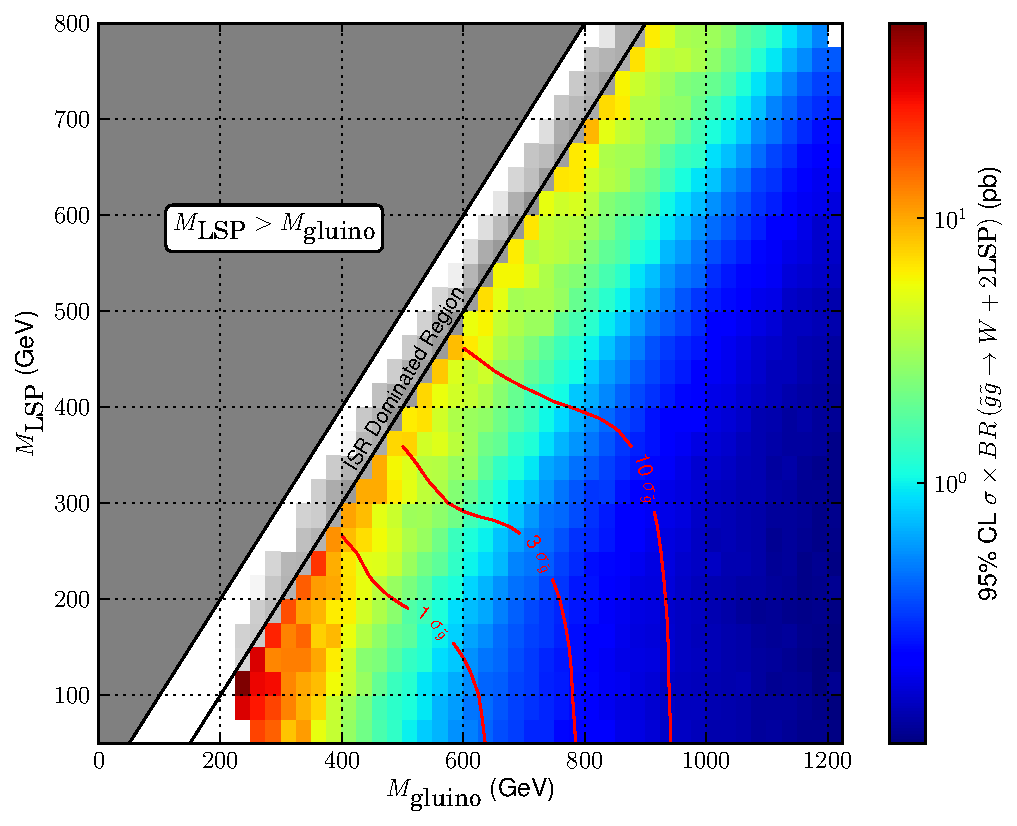
\includegraphics[width=0.49\textwidth]{fig/t3w_0p50_limit_sigsyst}}
\subfloat[]{\label{fig:inter_t3w_0p50_limit_1d}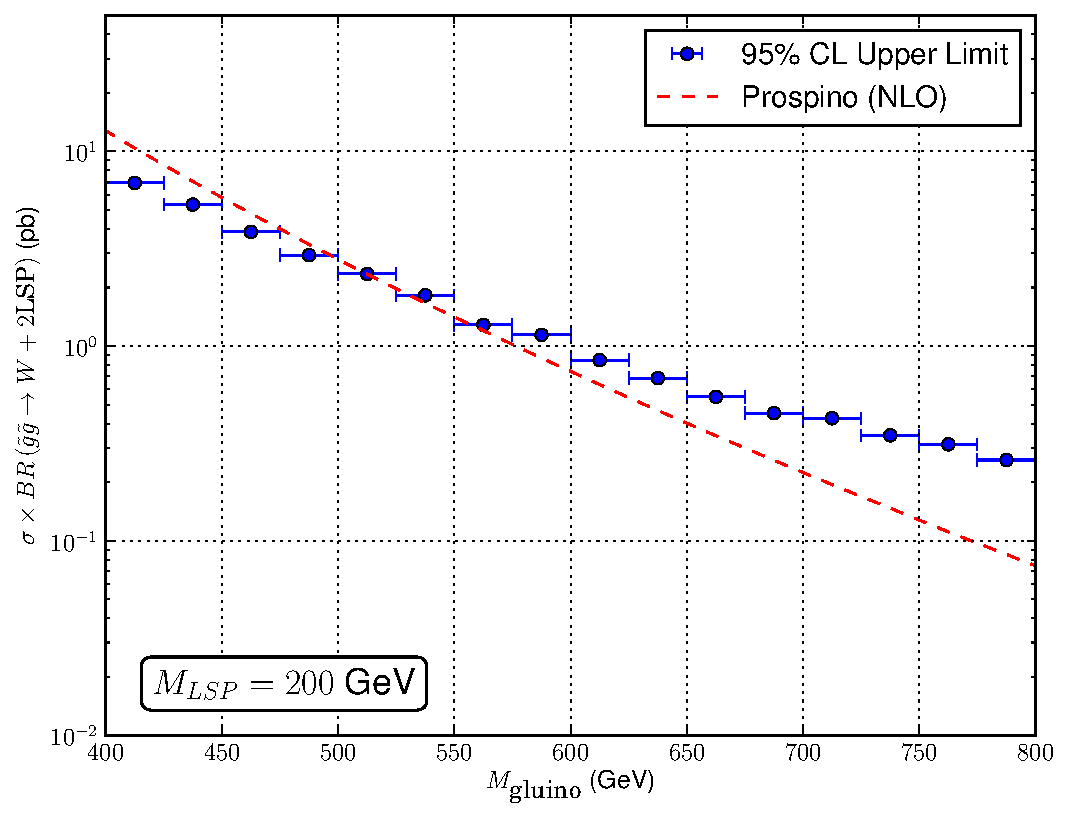
\includegraphics[width=0.49\textwidth]{fig/t3w_0p50_limit_sigsyst_1d}}
\caption[Limit in the \TthreeW simplified model with \Mchargino set assuming
$x=0.5$]{Limit in the \TthreeW simplified model with \Mchargino set assuming
  $x=0.5$. The 95\% confidence level upper limit on the cross-section as a
  function of $(\Mgluino, \Mlsp$) is shown in
  \subref{fig:inter_t3w_0p25_limit}. Overlayed are contours showing this
  exclusion in terms 1, 3 and 10 times the gluino cross-section predicted by
  \ac{QCD}. \fig~\subref{fig:inter_t3w_0p25_limit_1d} shows the same upper limit
  as a function of \Mgluino with $\Mlsp = \unit{50}{\GeV}$. Overlayed is the
  \ac{QCD} cross-section for gluino production.}
\label{fig:inter_t3w_0p50}
\end{figure}

\begin{figure}[h!]
\centering
\subfloat[]{\label{fig:inter_t3w_0p25_limit}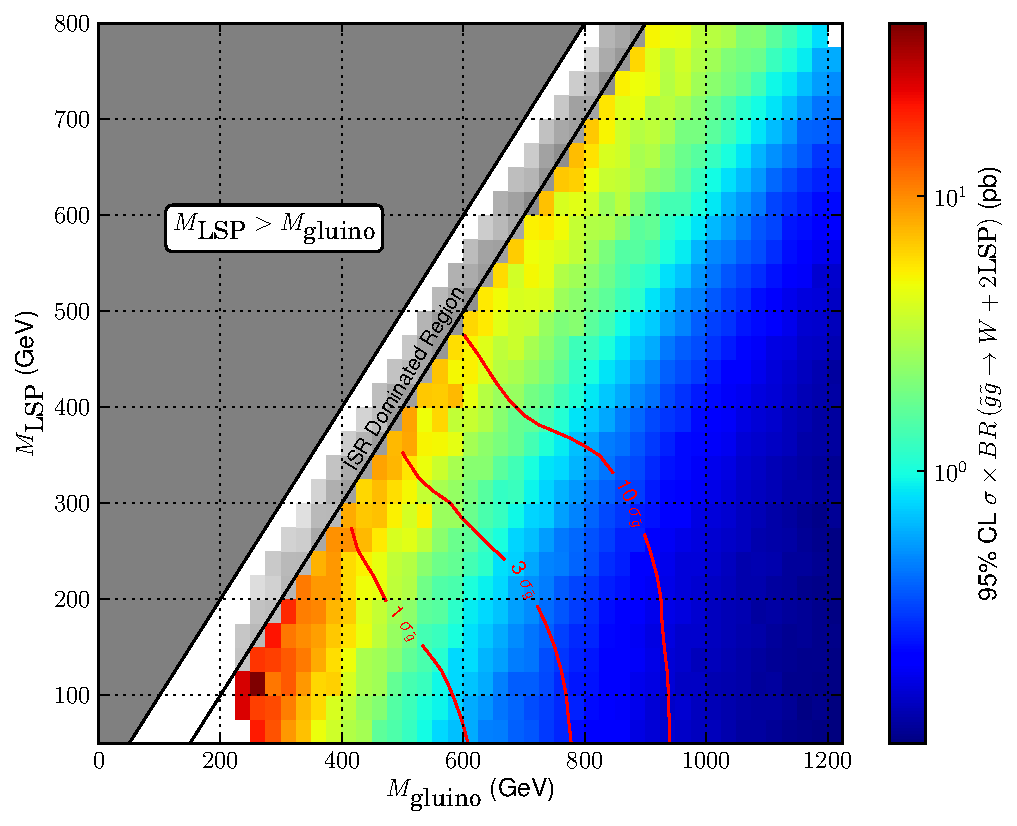
\includegraphics[width=0.49\textwidth]{fig/t3w_0p25_limit_sigsyst}}
\subfloat[]{\label{fig:inter_t3w_0p25_limit_1d}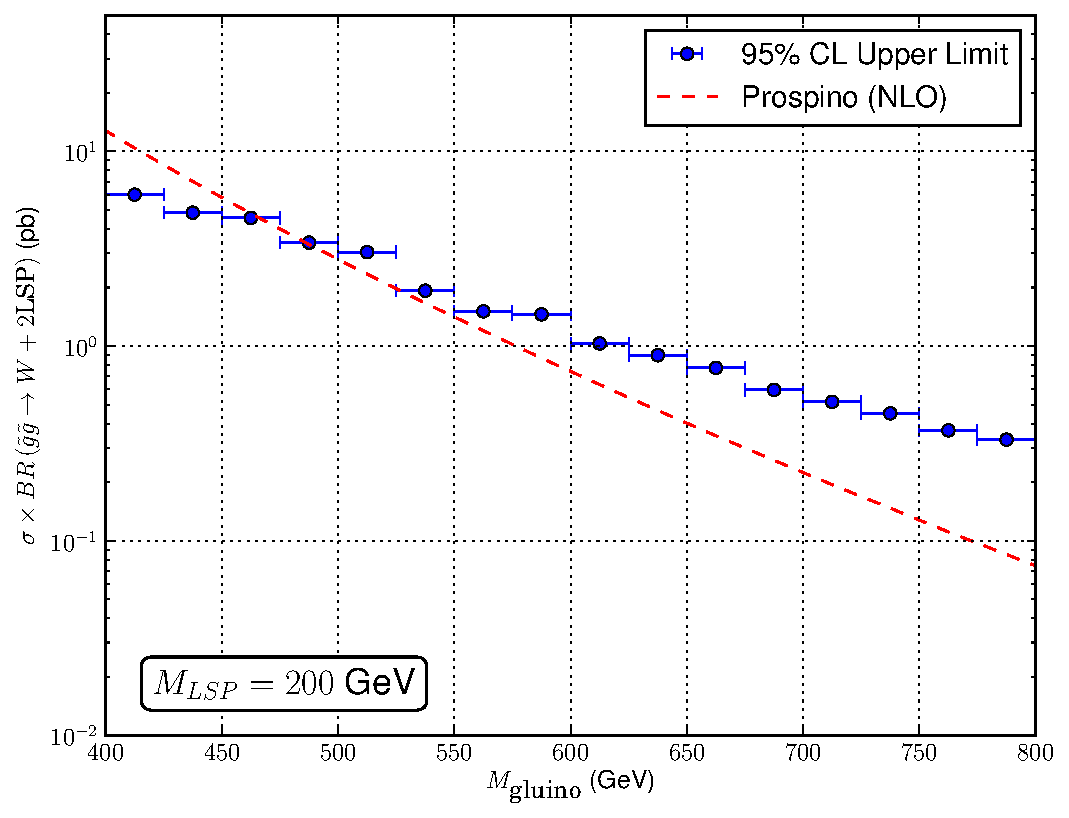
\includegraphics[width=0.49\textwidth]{fig/t3w_0p25_limit_sigsyst_1d}}
\caption[Limit in the \TthreeW simplified model with \Mchargino set assuming
$x=0.75$]{Limit in the \TthreeW simplified model with \Mchargino set assuming
  $x=0.75$. The 95\% confidence level upper limit on the cross-section as a
  function of $(\Mgluino, \Mlsp$) is shown in
  \subref{fig:inter_t3w_0p25_limit}. Overlayed are contours showing this
  exclusion in terms 1, 3 and 10 times the gluino cross-section predicted by
  \ac{QCD}. \fig~\subref{fig:inter_t3w_0p25_limit_1d} shows the same upper limit
  as a function of \Mgluino with $\Mlsp = \unit{50}{\GeV}$. Overlayed is the
  \ac{QCD} cross-section for gluino production.}
\label{fig:inter_t3w_0p25}
\end{figure}


\subsubsection{\Ttwott}
The \Ttwott model, as previously discussed, is of theoretical interest for
describing \ac{SUSY} theories with light stop squarks.

Efficiencies for each point in the $(\Mstop, \Mlsp)$ plane are shown in
\figs~\ref{fig:inter_t2tt_mu} and \ref{fig:inter_t2tt_el} for muons and
electrons respectively. Efficiencies are shown per \STlep bin in order to gauge
the effect of this cut on the efficiency.

\begin{figure}[h!]
\centering
\subfloat[$250 < \STlep < 350$]{\label{fig:inter_t2tt_mu_eff250}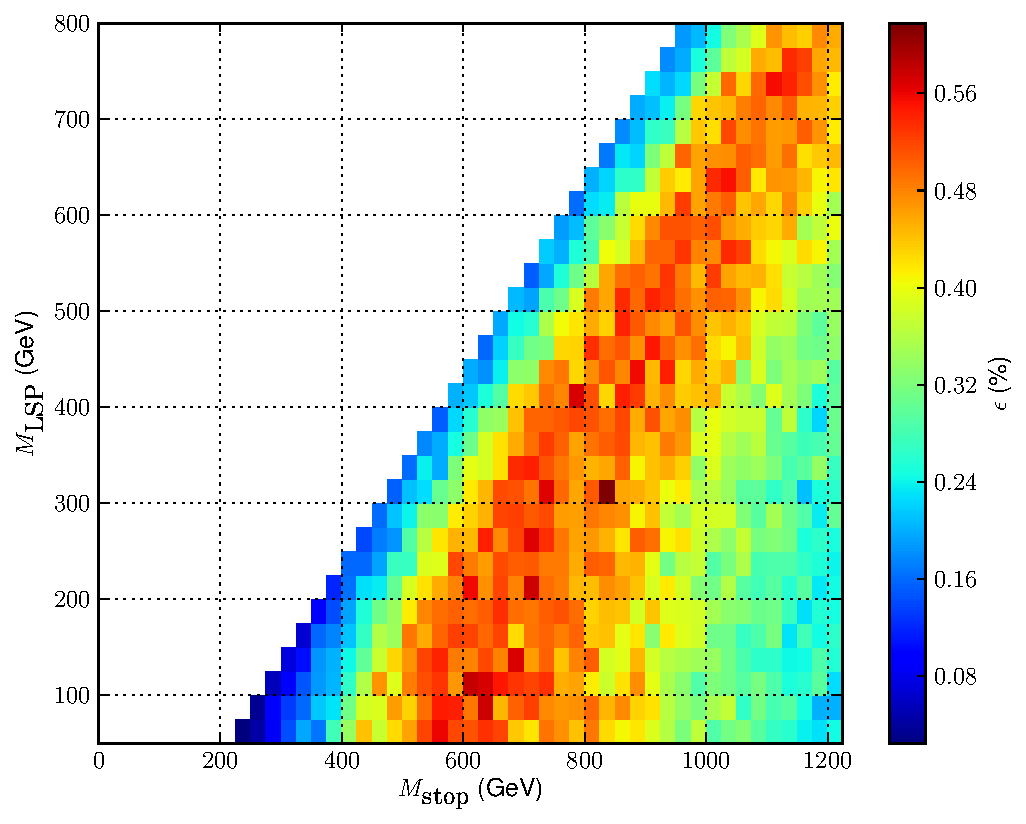
\includegraphics[width=0.43\textwidth]{fig/t2tt_muons_eff_250}}\quad
\subfloat[$350 < \STlep < 450$]{\label{fig:inter_t2tt_mu_eff350}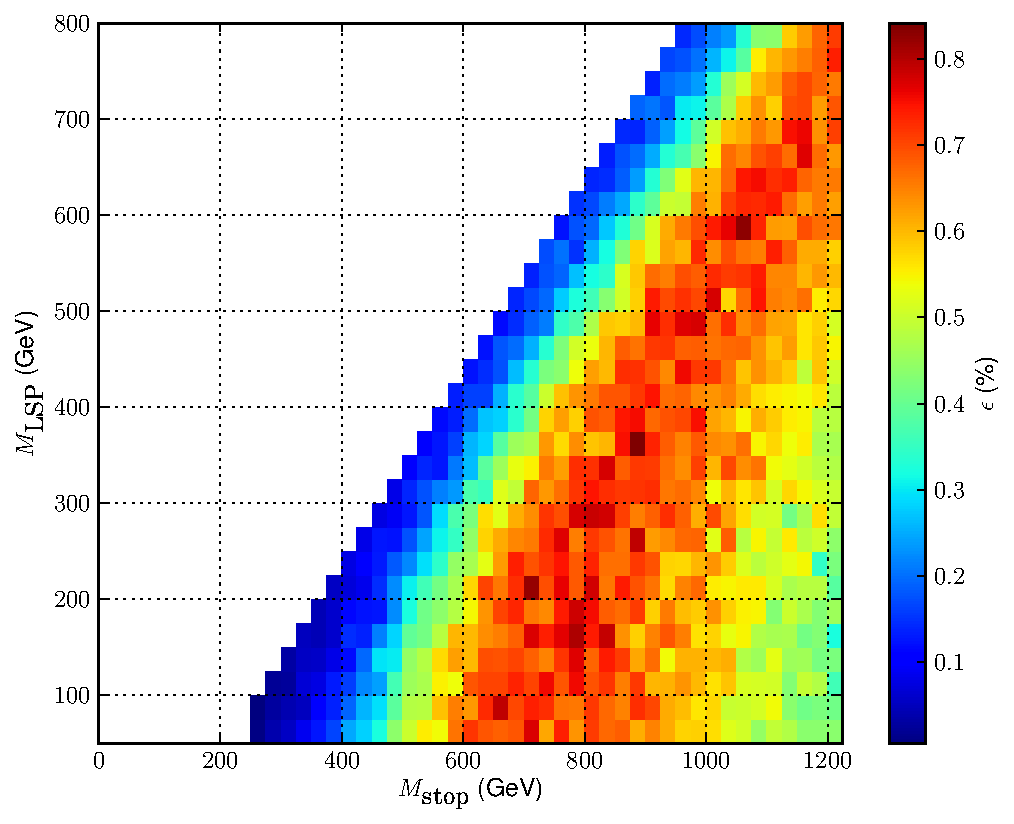
\includegraphics[width=0.43\textwidth]{fig/t2tt_muons_eff_350}}\\
\subfloat[$\STlep > 450$]{\label{fig:inter_t2tt_mu_eff450}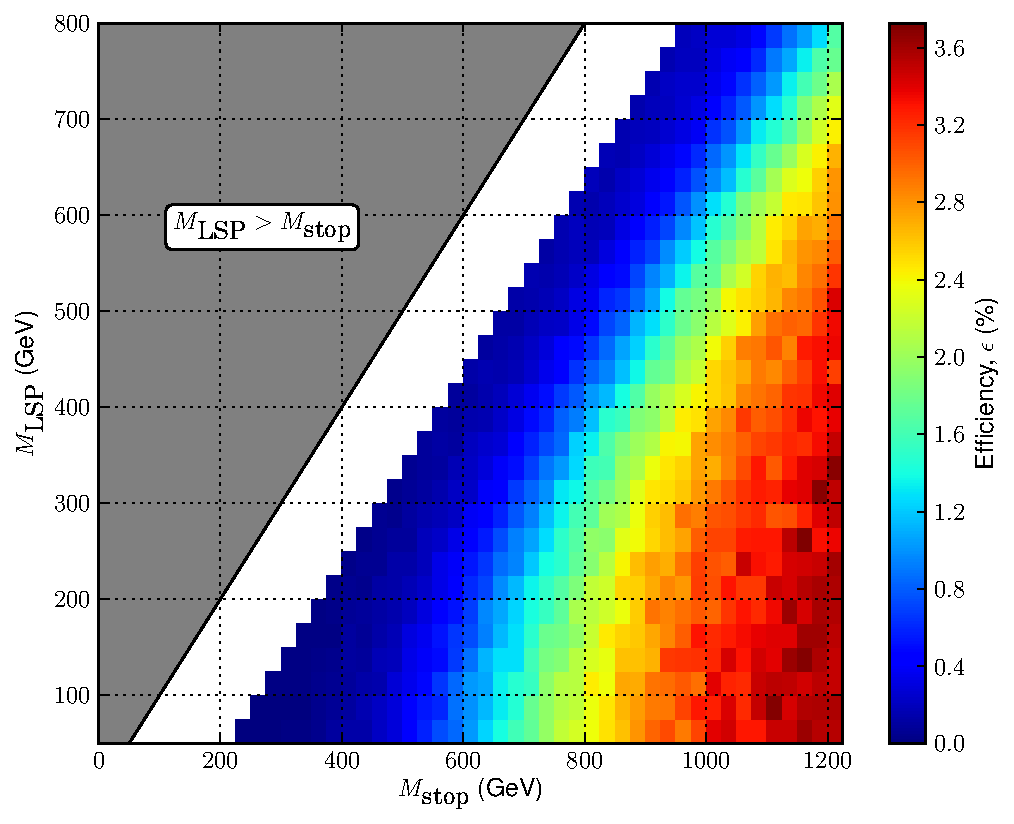
\includegraphics[width=0.43\textwidth]{fig/t2tt_muons_eff_450}}\quad
\subfloat[Total]{\label{fig:inter_t2tt_mu_efftot}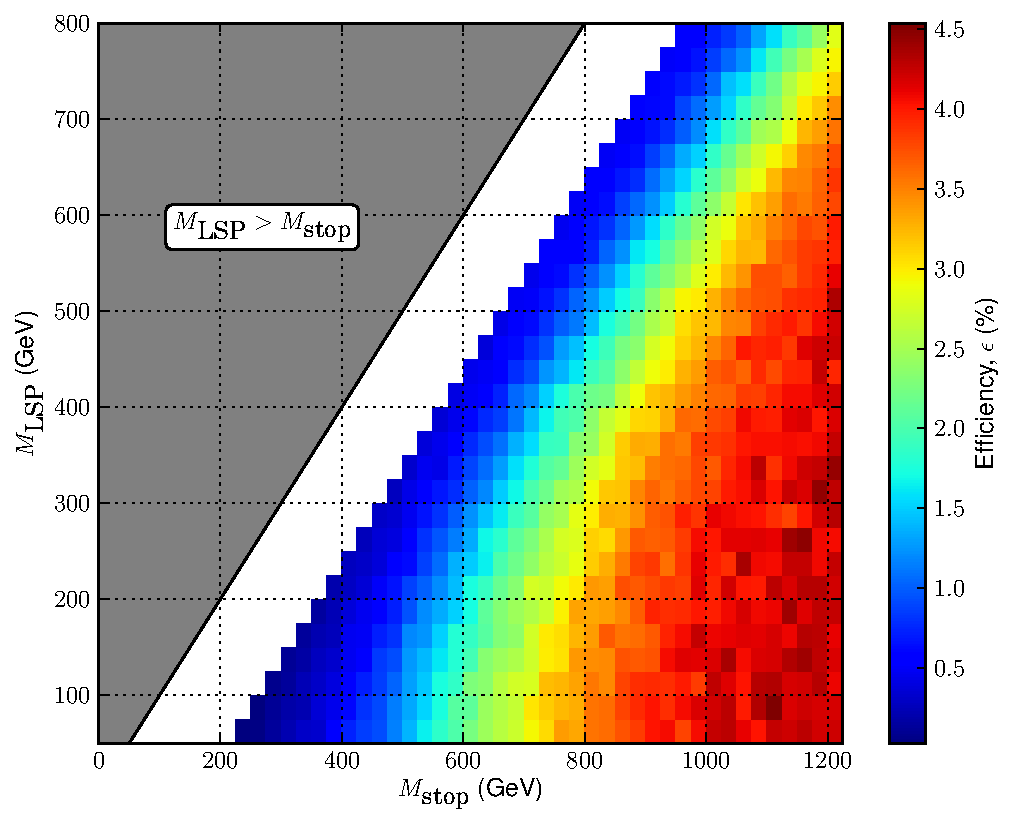
\includegraphics[width=0.43\textwidth]{fig/t2tt_muons_eff_total}}
\caption[Signal efficiency maps for the muon channel in the \Ttwott simplified
  model]{Signal efficiency maps for the muon channel in the \Ttwott simplified
  model. Efficiency is shown as a function of $(\Mstop, \Mlsp)$ for each \STlep
  bin and for the total across all three bins.}
\label{fig:inter_t2tt_mu}
\end{figure}

\begin{figure}[h!]
\centering
\subfloat[$250 < \STlep < 350$]{\label{fig:inter_t2tt_el_eff250}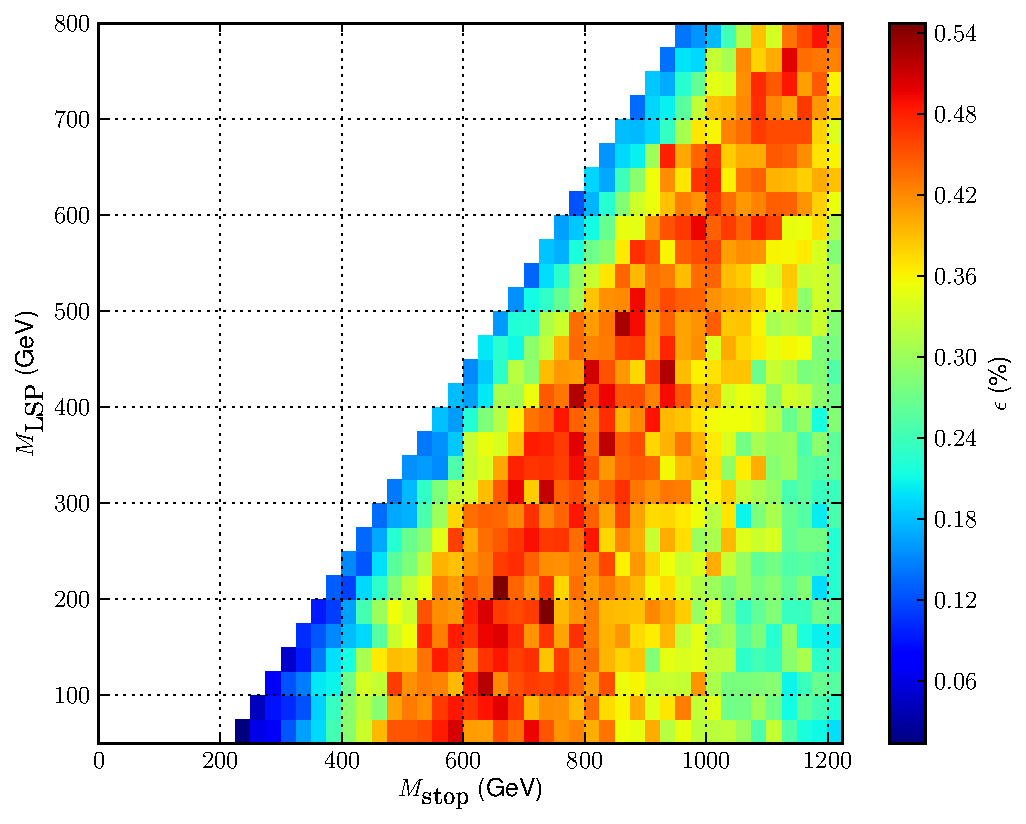
\includegraphics[width=0.43\textwidth]{fig/t2tt_electrons_eff_250}}\quad
\subfloat[$350 < \STlep < 450$]{\label{fig:inter_t2tt_el_eff350}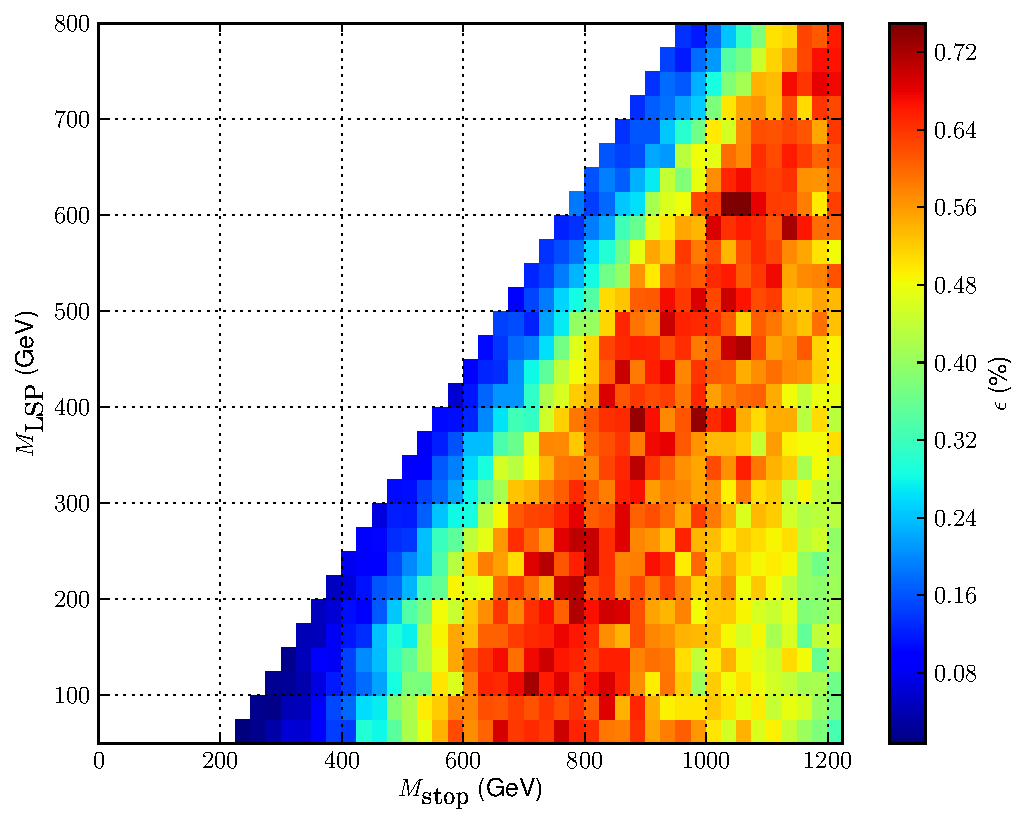
\includegraphics[width=0.43\textwidth]{fig/t2tt_electrons_eff_350}}\\
\subfloat[$\STlep > 450$]{\label{fig:inter_t2tt_el_eff450}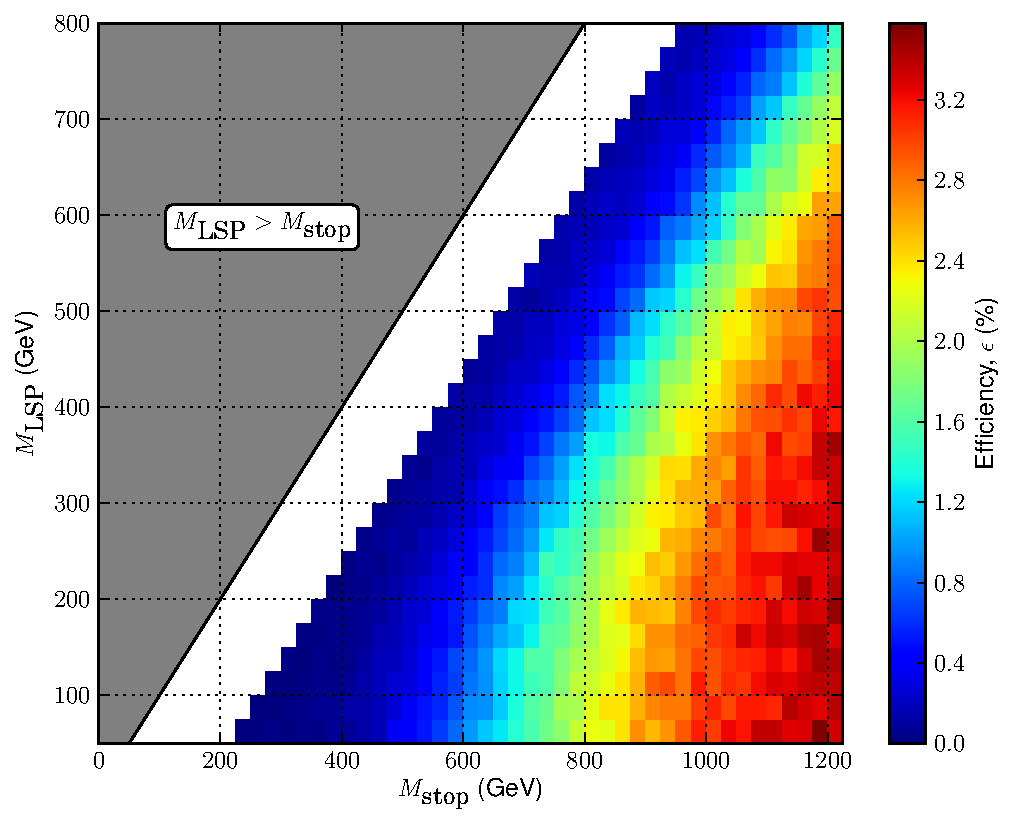
\includegraphics[width=0.43\textwidth]{fig/t2tt_electrons_eff_450}}\quad
\subfloat[Total]{\label{fig:inter_t2tt_el_efftot}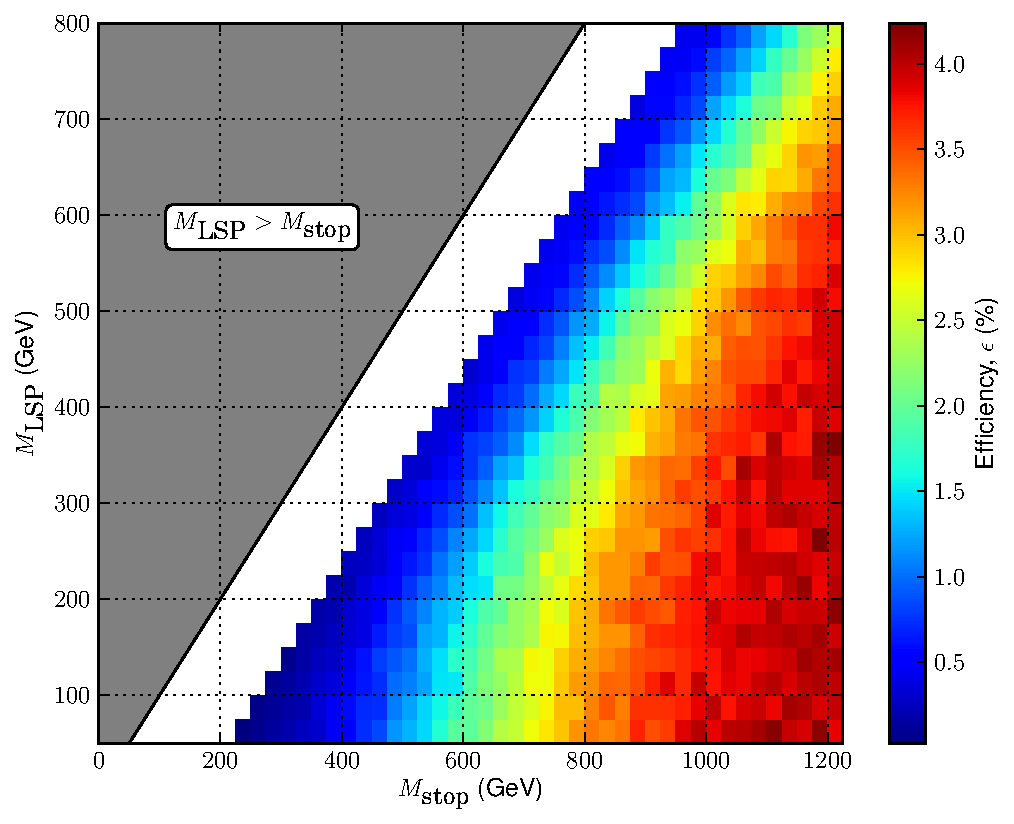
\includegraphics[width=0.43\textwidth]{fig/t2tt_electrons_eff_total}}
\caption[Signal efficiency maps for the electron channel in the \Ttwott simplified
  model]{Signal efficiency maps for the electron channel in the \Ttwott simplified
  model. Efficiency is shown as a function of $(\Mstop, \Mlsp)$ for each \STlep
  bin and for the total across all three bins.}
\label{fig:inter_t2tt_el}
\end{figure}

The observed limit is shown in a similar fashion to the \TthreeW case in
\fig~\ref{fig:inter_t2tt}. It can be seen that no exclusion is possible with
respect to the stop cross-section predicted by \ac{QCD}. It is possible that a
dedicated search using B-tagged jets would provide significantly improved
sensitivity.

\begin{figure}[h!]
\centering
\subfloat[]{\label{fig:inter_t2tt_limit}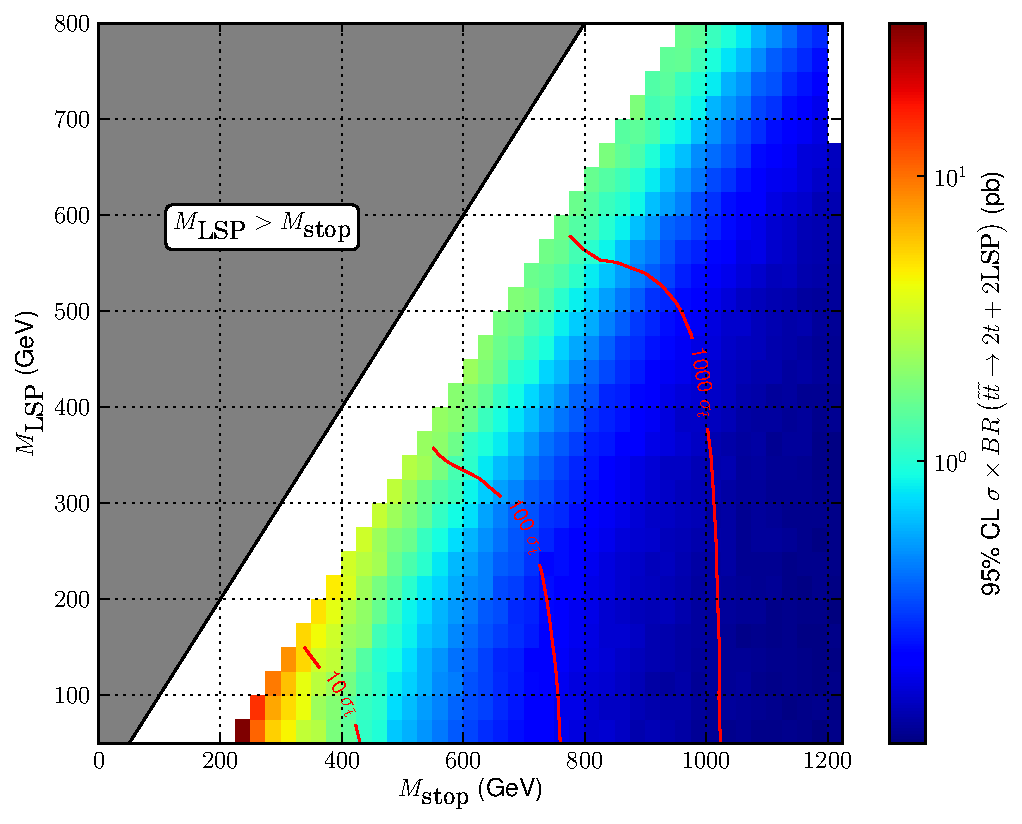
\includegraphics[width=0.49\textwidth]{fig/t2tt_limit_sigsyst}}
\subfloat[]{\label{fig:inter_t2tt_limit_1d}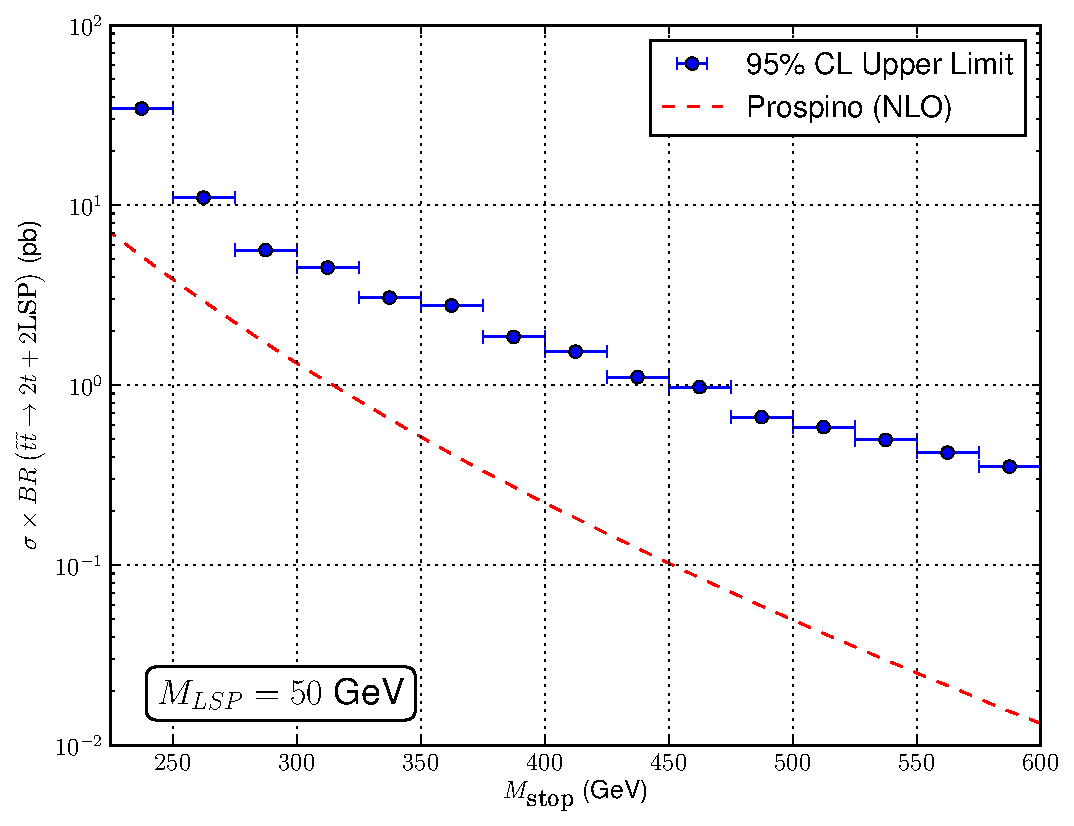
\includegraphics[width=0.49\textwidth]{fig/t2tt_limit_sigsyst_1d}}
\caption[Limit in the \Ttwott simplified model]{Limit in the \Ttwott simplified
  model. The 95\% confidence level upper limit on the cross-section as a
  function of $(\Mstop, \Mlsp$) is shown in
  \subref{fig:inter_t3w_0p25_limit}. The overlayed contours show this exclusion
  in terms of 1, 10 and 1000 times the stop production cross-section predicted
  by \ac{QCD}. The upper limit is shown as a function of \Mstop in
  \subref{fig:inter_t2tt_limit_1d} for $\Mlsp = \unit{50}{\GeV}$. }
\label{fig:inter_t2tt}
\end{figure}

\section{Summary}
The single lepton supersymmetry search detailed in \chap~\ref{sec:susysearch}
has been interpreted within the context of several models. A likelihood function
has been developed which embodies all significant statistical and systematic
uncertainties. The \CLs procedure has been used to calculate an excluded region
in the \ac{CMSSM}. The single lepton supersymmetry search is seen to exclude a
significant portion of the parameter space.

Additionally, two simplified models have been investigated: \TthreeW and
\Ttwott. The \ac{PL} method has been used to set an upper limit as a function of
the model parameter space in each case. This has also been compared to a
cross-section calculation, assuming \ac{QCD}-strength coupling. In the \TthreeW
case, significant regions of the parameter space have been excluded. The \Ttwott
model is of theoretical interest from the perspective of \ac{SUSY} models
containing a light stop squark. In this case, the sensitivity of this particular
analysis is seen to be limited. Sensitivity could be enhanced with the addition
of \Pbottom-tagged jets to the analysis. This could be an interesting avenue for
future study.



%%% Local Variables:
%%% mode: latex
%%% TeX-master: "../thesis"
%%% End:
